\documentclass[conference]{IEEEtran}


  	\usepackage[pdftex]{graphicx}
  	\graphicspath{{../pdf/}{../jpeg/}}
	\DeclareGraphicsExtensions{.pdf,.jpeg,.png}
	\usepackage{subcaption}

	\usepackage[cmex10]{amsmath}
	\usepackage{mathabx}
	\usepackage{algorithmic}
	\usepackage{array}
	\usepackage{mdwmath}
	\usepackage{mdwtab}
	\usepackage{eqparbox}
	\usepackage{url}
	\hyphenation{op-tical net-works semi-conduc-tor}

\pagestyle{plain}

\begin{document}

\begin{titlepage}
\begin{centering}
\newcommand{\HRule}{\rule{\linewidth}{0.5mm}}
\vspace*{\fill}

\includegraphics[width=200pt]{images/Logo_EPFL.png}

\smallskip

\textsc{\Large Master Semester Project in Electrical Engineering}
\vspace{0.5cm}\\

\HRule \\ [0.4cm]
\huge \textbf{Deep neural method for SIM super-resolution reconstruction with a reduced number of images}
\smallskip
\HRule \\[0.3cm]
\vspace*{\fill}
\Large 10 ECTS
\vspace*{\fill}
\Large{\textit{\\Author:}}\\
\Large Kay \textsc{Lächler} (MA3 EL)

\bigskip

\medskip

\Large{\textit{\\Supervisors:}}\\
\Large{Daniel \textsc{Sage} (Biomedical Imaging Group)\\\&\\Emmanuel \textsc{Soubies} (Toulouse, France)}\\

\vspace*{\fill}

\large Autumn 2020 --- EPFL

\end{centering}
\end{titlepage}

\begin{abstract}
In this project an alternative to the classical 9-image SR-SIM reconstruction method was proposed using 4-image SR-SIM paired with a DNN. It allows to compensate for the typical reconstruction artefacts and provide a noise resistant, clean super-resolution image. The implemented system requires only 3 raw structured images and a widefield image, reducing acquisition time and photobleaching effects. The appropriate DNN architecture for this task was found to be RCAN. It was trained on simulated SIM images using the DIV2K dataset. A detailed evaluation, using several metrics on three simulated SIM test images with different noise levels confirmed that the proposed system could indeed provide super-resolution images from a reduced number of SIM images.
\end{abstract}

\section{Introduction}
Microscopic image acquisition systems are characterised by their unique point spread function (PSF) that depends on different parameters, including the lens and the sample medium. Consequently, the acquired image is a convolution of the original point source with the system's PSF, which in the frequency domain, corresponds to a multiplication by the optical transfer function (OTF). The OTF usually is an Airy disk \cite{airy1835diffraction} of finite radius, meaning that some of the high frequency components are lost during the imaging process, resulting in a blurred version of the original point source. Moreover, in 1873, Ernst Abbe had shown that even with the best possible acquisition system, the diffraction of light poses an upper limit on the resolution that can be achieved with classical widefield (WF) fluorescence microscopy \cite{Fluorescence_microscopy}, given by the expression $\frac{\lambda}{2\operatorname{NA}}$, with $\lambda$ the emitted wavelength and $\operatorname{NA}$ the numerical aperture, which lies around 200nm for typical wavelengths used in fluorescent imaging (400-700nm \cite{ZEISS_wavelengths}).

\subsection{Super-Resolution Structured Illumination Microscopy}

A direct method to overcome this diffraction limit by using \textbf{S}uper-\textbf{R}esolution \textbf{S}tructured \textbf{I}llumination \textbf{M}icroscopy (\textbf{SR-SIM}) was developed around 20 years ago by Heintzmann and Cremer \cite{Heintzmann_diffraction_grating} as well as Gustafsson \cite{Gustafsson_orig}. In SR-SIM, the idea is to mix the otherwise undetectable high frequency components into the low frequency space, such that they can be acquired with a conventional light microscope. To this end, instead of using a uniform illumination, the sample is illuminated with a sinusoidal illumination pattern, given by 
$$I(r)=I_0[1+\cos(k_0r+\phi)]$$
with $I_0$ the illumination amplitude, $k_0$ the wave vector and $\phi$ the phase offset. Illuminating the sample with such a pattern results in the formation of so called Moiré fringes \cite{moire_fringes_paper}, which in the frequency space, corresponds to shifting high frequency components into low frequency space. The shifted amount directly depends on the grating period of the illumination pattern, so by choosing a grating period similar to the diffraction limit of the acquisition system, the final image resolution can in theory be doubled. The resulting composite Fourier transform (FT) is then unmixed and reconstructed as illustrated in figure \ref{fig:zeiss_sim}.

\begin{figure}[h]
    \centering
    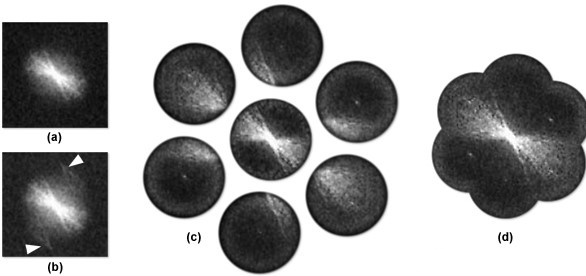
\includegraphics[width=0.48\textwidth]{images/Inkedzeiss_sim_showcase_LI.jpg}
    \caption{Representation of the SR-SIM reconstruction in the frequency space. FT of the widefield image (a), composite FT of one of the SR-SIM images indicating the mixed frequency components (b), unmixed FTs of all SR-SIM images (c) and reconstructed FT of the super-resolved image (d). Figure taken from ZEISS Microscopy Online Campus \cite{zeiss_sim}. The original image was created by Gustafsson \cite{Gustafsson_orig}.}
    \label{fig:zeiss_sim}
\end{figure}

Current 2D SR-SIM systems usually acquire 9 separate images composed of 3 different phase offsets for each of the 3 differently oriented illumination patterns. Importantly, all illumination patterns need to be independent from each other and span the entire frequency spectrum. Such a reconstruction is either integrated in the microscope software itself or can be performed by using external tools like fairSIM \cite{fairsim_article}. While this method generally delivers good results, acquiring 9 images to create one single image is time consuming and encourages photobleaching\footnote{"Photobleaching is the chemical alteration of the indicator dye [...], so that it is unable to fluoresce due to the destruction of covalent or non-covalent bonds due to non-specific binding caused by excitation light." \cite{OMARA2018130}}. Additionally, it can also create unwanted artefacts in the case of a low signal-to-noise ratio in the raw SIM images or as a result of bad calibration, as illustrated in figure \ref{fig:sim_artefacts_showcase}. In fact, although there exist automatic parameter estimation algorithms, the exact parameters have to be tuned manually for every single image in order to obtain the best results. For these reasons in recent years and especially last year, there have been numerous projects that use deep neural networks in order to either speed up the process or to improve the noise- and parameter-change resistance of the reconstruction.

\begin{figure}[h]
    \centering
    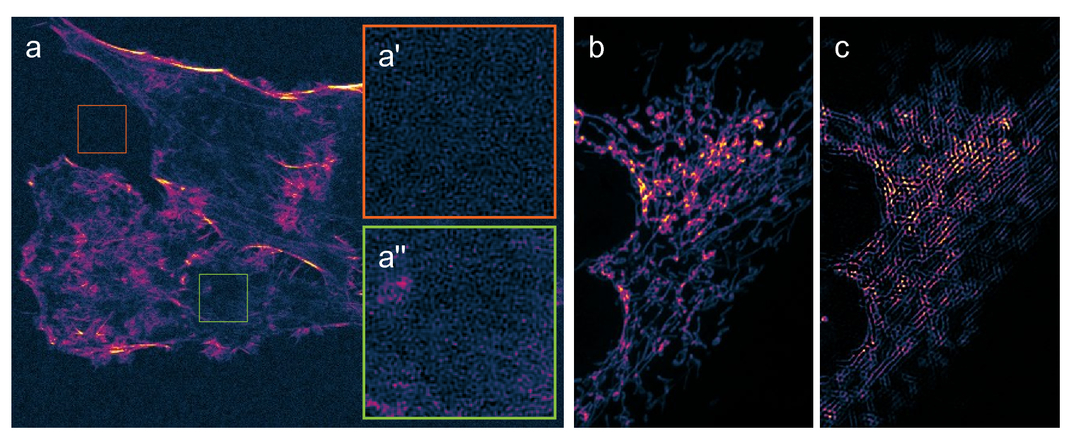
\includegraphics[width=0.48\textwidth]{images/sim_artecats_showcase.jpg}
    \caption{Example of common SIM artefacts. Image taken from \cite{sim_artefacts_paper}. Original SIM image (a), background artefacts (a'), object artefacts (a''), a well reconstructed SIM image (b) and the same SIM image that was reconstructed with a slight OTF mismatch (c).}
    \label{fig:sim_artefacts_showcase}
\end{figure}

\subsection{State of the Art}
In 2020, three independently released papers have made interesting advancements on the topic of using a deep neural network (DNN) to improve on the classic SR-SIM reconstruction method. The Widefield2SIM (W2S) EPFL project \cite{W2S_paper} focused on training a DNN to directly map a widefield image to a super-resolution image, without any actual structured illumination involved. The obvious advantage of this approach is its rapid acquisition time, since only one image with a uniform illumination has to be generated. However, while producing good-looking images, the reliability of converting a low resolution image to a super-resolved image without actually having any additional information on the high frequency components is questionable for biologists.

The ML-SIM project \cite{mlsim_paper} took a different approach and created an end-to-end DNN that incorporates the whole SR-SIM reconstruction pipeline. It takes as input the raw SIM stack of 9 images and generates the super-resolved image. This method not only delivers better results than the fairSIM reconstruction algorithm in good conditions, but it's also more resistant to noise. Furthermore, the ML-SIM network can also be trained with a reduced number of images, speeding up the acquisition process at the cost of image quality.

Lastly, a recent paper from October 2020 studied two DNNs called RED-Net and SR-REDSIM \cite{sr-redsim_paper}. The latter is also an end-to-end network, much like the one used in ML-SIM however, this one used real SIM images as the training set instead of simulated ones. The RED-Net on the other hand has been trained to improve the output of the fairSIM reconstruction method. As such it's not an end-to-end network like the others but takes the SR-SIM image created by fairSIM and enhances it to reduce artefacts, improve the resistance to noise and system parameter fluctuations and improve the overall image quality.

Especially this last version presents a promising idea, since it relies on the classic reconstruction method, which is based on the knowledge we have about how the high frequency components are mixed in SIM images. The main advantage of this approach is the ability to easily change the reconstruction parameters from one image to another, unlike in an end-to-end DNN, while also addressing the weaknesses of the classic method. The only issue is that the fairSIM algorithm used by this method only works with at least 9 raw SIM images, thus offering no gain in acquisition speed.

\subsection{Aim of this project}
In this project, the goal was to combine both the reliability of the classic reconstruction algorithm with the flexibility and performance of a DNN, as well as speed up the acquisition process by working with a reduced number of SIM images. The DNN was used as the end stage of a pre-existing, imperfect 4-image SR-SIM reconstruction algorithm, with the hope that it would be able to compensate for the large amount of artefacts created, especially at low signal-to-noise ratios. The implementation and training of the DNN was the main part of this project, but a large amount of work also went into the exploration of different datasets, creating a pipeline for the simulation of raw SIM images with different noise levels and finding representative metrics for comparing the results.

\section{Method}
\subsection{4-Image SR-SIM Reconstruction Algorithm}
The 4-image SR-SIM reconstruction algorithm used to create the training images for the DNN was derived by Christophe Muller in 2018 \cite{muller_project} and exploits the redundancy found in the classic 9-image reconstruction. While there exists a fast direct method for the 9-image reconstruction algorithm, the 4-image reconstruction uses a slower, iterative approach. The four images used by this algorithm consist of three SIM images with independent orientations and one widefield image. The phase offset of the illumination patterns are not important and can be chosen arbitrarily.

It should be noted that the current version of this algorithm only works correctly when using simulated SIM images with a perfect PSF, meaning that the results obtained cannot be generalized for real SIM images.

\subsection{DNN Structure and loss function}
To create and train the DNN, the Python library pytorch \cite{PyTorch_website} was used. The first implementations of the DNN were created by using the popular U-Net structure \cite{ronneberger2015unet}. This convolutional network structure was originally created for image segmentation, but has since been adapted to various other image processing tasks. It consists of a downscaling pathway, followed by an upscaling pathway, each one with several intermediate steps where skip connections connect the two pathways. This specific structure creates a "multiscale" network, meaning that the image is processed at multiple resolutions in parallel and then the extracted information from all resolutions is combined to create the output image.

\begin{figure}[h!]
    \centering
    \begin{subfigure}[b]{0.15\textwidth}
        \centering
        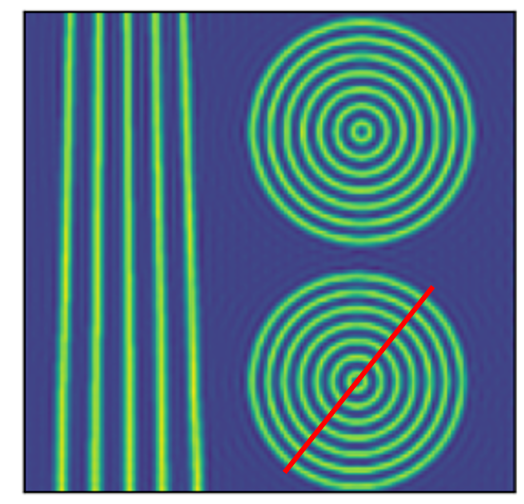
\includegraphics[width=\textwidth]{images/gt_circle_line.png}
        \caption{Ground-Truth}
        \label{fig:gt_circle}
    \end{subfigure}
    \begin{subfigure}[b]{0.151\textwidth}
        \centering
        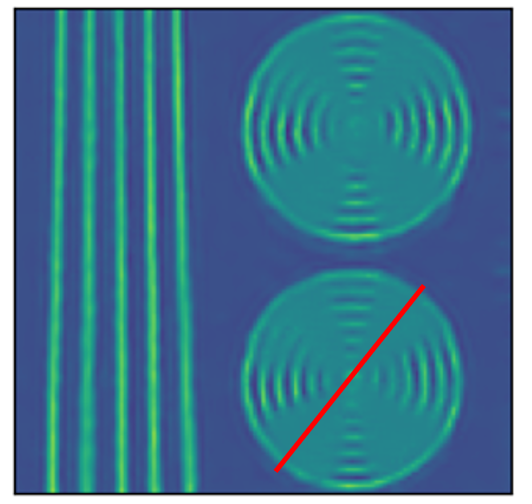
\includegraphics[width=\textwidth]{images/unet_circle_line.png}
        \caption{U-Net}
        \label{fig:unet_circle}
    \end{subfigure}
    \begin{subfigure}[b]{0.145\textwidth}
        \centering
        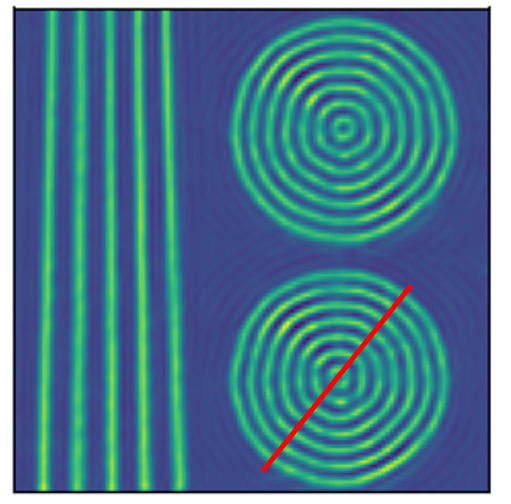
\includegraphics[width=\textwidth]{images/rcan_circle_line.png}
        \caption{RCAN}
        \label{fig:rcan_circle}
    \end{subfigure}
    \begin{subfigure}[b]{0.15\textwidth}
        \centering
        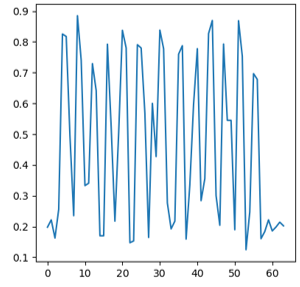
\includegraphics[width=\textwidth]{images/gt_circle_cut.png}
        \caption{GT profile}
        \label{fig:gt_circle_cut}
    \end{subfigure}
    \begin{subfigure}[b]{0.153\textwidth}
        \centering
        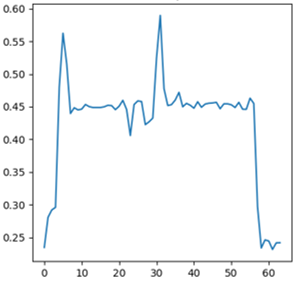
\includegraphics[width=\textwidth]{images/unet_circle_cut.png}
        \caption{U-Net profile}
        \label{fig:unet_circle_cut}
    \end{subfigure}
    \begin{subfigure}[b]{0.149\textwidth}
        \centering
        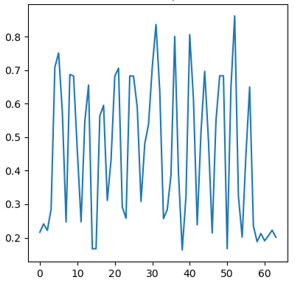
\includegraphics[width=\textwidth]{images/rcan_circle_cut.png}
        \caption{RCAN profile}
        \label{fig:rcan_circle_cut}
    \end{subfigure}
    \caption{Original image (a), U-Net output (b) and RCAN output (c) of the thin circle feature from one of the test images. (d), (e) and (f) show the corresponding intensity profiles across the diagonal of the bottom thin circle feature, indicated by the red line.}
    \label{fig:circle_comp}
\end{figure}

Initially, this structure looked promising until one of the test images revealed a fatal flaw in the output images of this DNN. Looking at figure \ref{fig:circle_comp}, we can see that the U-Net is not capable of correctly reconstructing the diagonals of the thin circles, but has no problem doing so for the horizontal and vertical orientations. As the line profiles in the bottom half of the figure show, the individual circles cannot be distinguished at an angle of around $\pm45^\circ$. The reason for this behaviour could not be determined with certainty, but is possibly connected to the multiscale structure of the U-Net and/or the non-isotropy of the small $3\times 3$ kernels that might not treat all orientations equally.

\begin{figure}[h]
    \centering
    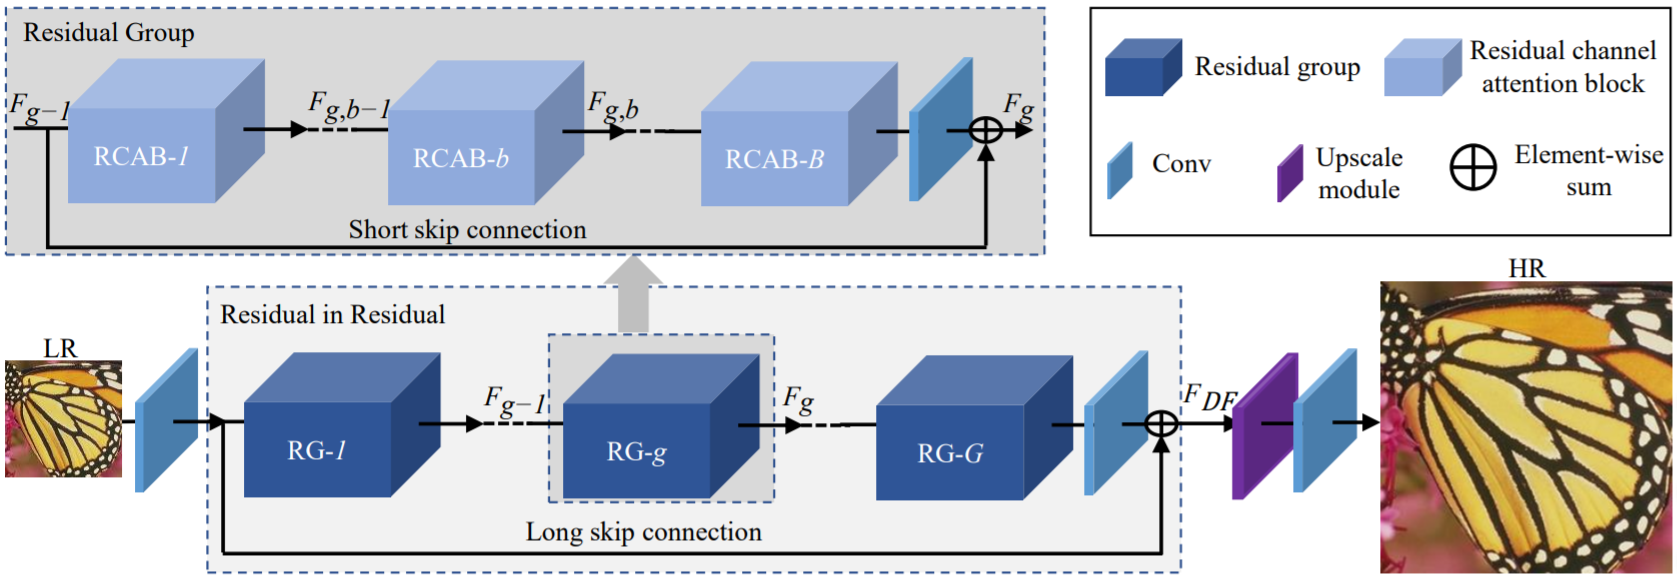
\includegraphics[width=0.48\textwidth]{images/rcan_structure.png}
    \caption{Illustration depicting the RCAN structure, containing several residual groups with several residual channel attention blocks each. Image taken from the original RCAN paper \cite{zhang2018rcan}.}
    \label{fig:rcan_structure}
\end{figure}

For this reason, later implementations of the DNN adapted the residual channel attention network (RCAN) structure \cite{zhang2018rcan} depicted in figure \ref{fig:rcan_structure}, which was developed in 2018 to perform single image super resolution and was shown to outperform state of the art methods. The RCAN structure adapted for this project consisted of 3 residual groups, each one containing 5 residual channel attention blocks. In each residual channel attention block (RCAB), 64 features were first produced using global average pooling that were then further processed by reduction and extension. Finally a skip connection was used to multiply the RCAB input with the resulting features. The resulting network includes 159 layers with a total of 1'265'469 trainable parameters. In comparison to the U-Net, which consisted of 45 layers and a total of 31'030'593 trainable parameters, the RCAN network is much deeper but has considerably less trainable parameters. The preliminary results obtained showed that the RCAN structure delivers consistently better results, suggesting that for this task, the depth of the network might be more important than the number of trainable parameters.

As for the loss function, a combination of the structure similarity index measure (SSIM) \cite{ssim_article} and the smooth L1 loss (sL1) was used:
$$L=\alpha(1-\operatorname{SSIM})+(1-\alpha)\operatorname{sL1}$$
This specific combination, with $\alpha=0.84$, was shown to be optimal in training a DNN for image restoration \cite{loss_func_comp_paper}, which was confirmed and thus adapted in this project.

\subsection{Dataset}
\label{sec:Dataset}
For the training and validation images the popular computer vision dataset DIV2K \cite{Agustsson_2017_CVPR_Workshops, Timofte_2017_CVPR_Workshops, Ignatov_2018_ECCV_Workshops} was used. This dataset consists of 900 high-resolution images gathered from the internet.

In a first step, the images were cropped to be square and resized to $1024\times 1024$ pixels. From these non-microscopy related images, the raw SIM images were simulated by first multiplying them with the corresponding illumination patterns, then performing a convolution with an ideal PSF and finally adding the desired amount of noise. The simulated illumination wavelength was $\lambda=488$nm, the numerical aperture $\operatorname{NA}=1.4$, the refractive index of the objective medium (glass / oil) $\operatorname{nl}=1.51$ and the refractive index of the sample medium (water) $\operatorname{ns}=1.333$. The resolution was set to 32nm per pixel, meaning that a $1024 \times 1024$ image corresponds to a visible area of 32.768$\mu$m$^2$. With these parameters, the theoretical diffraction limit can be estimated at $\frac{\lambda}{2\operatorname{NA}}=174.3nm$.

\begin{figure}[h]
    \centering
    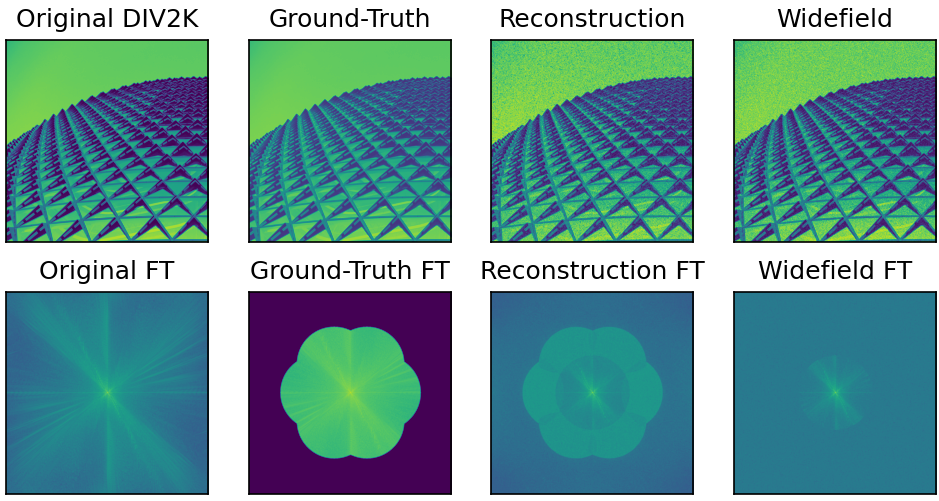
\includegraphics[width=0.48\textwidth]{images/images_and_FTs.png}
    \caption{From left to right: An original DIV2K image, its corresponding ground-truth, where the Fourier transform has been masked to simulate a perfect 9-image SR-SIM reconstruction, the net input (SNR=10dB), which is the output of the 4-image SR-SIM reconstruction algorithm and the simulated widefield image (SNR=10dB). The bottom images are the corresponding Fourier transforms.}
    \label{fig:images_and_FTs}
\end{figure}

Additionally to the SIM images, a widefield image was also simulated for each high-resolution image, which was for one used in the 4-image reconstruction process, but also served as a comparison for the reconstructed image. The simulated raw SIM stacks, together with the widefield image created by this method were then used as input to the 4-image SR-SIM reconstruction algorithm, which resulted in the final dataset consisting of 900 simulated SR-SIM images. 720 (80\%) of those images were used for training and 180 (20\%) were used for validation. The ground-truth images were created by masking the Fourier transform of the original DIV2K images in order to simulate a perfect 9-image SR-SIM reconstruction. This was done to stay as close to reality as possible, since the network should only be able to improve on the frequency components that are actually present in the image and not try to add any additional interpretation of the data. Figure \ref{fig:images_and_FTs} shows an example of the four types of images created during the dataset creation together with their Fourier transforms to illustrate the changes in both the space and frequency domain. The fact that the dataset consisted of non-microscopy images should ensure that the trained model doesn't show any preference for certain cell types or structures and thus the results can be generalized for any bio-imaging application.

It should be noted that during the training process, the dataset had to be split in two subsets of 450 images each because the server used for the training didn't have enough memory to work with the entire 7.5GB dataset at once. The training process was thus conducted in steps of 20 epochs, after which the datasets were switched and the training continued. Similarly, the maximum batch size that could be used without overflowing the GPU's memory was 2, which slowed down the training process, but shouldn't have any negative effect on the final result.

\subsection{Complete System}

The complete 4-image SR-SIM reconstruction system, including the reconstruction, correction by the DNN and any pre- and post-processing is shown in figure \ref{fig:system_block_diagram}. First, the raw SIM-stack of three SIM images and one widefield image are given to the 4-image SR-SIM reconstruction algorithm that is coded in MATLAB. The PSF is either created by the algorithm from the given parameters or provided by the user. The reconstruction algorithm iteratively approximates the illumination patterns and uses this information to unmix the frequency components and ultimately construct the super-resolved image. The output of the reconstruction output is then normalized to have zero mean and a standard deviation of 1. Next, the normalized 4-image reconstruction is fed into the DNN, coded in python, which performs the artefact correction and overall image improvement. Finally, the corrected image is converted to the desired intensity range (here [0,1]) and visualized with a suitable color-map (here "viridis").

\begin{figure}[h]
    \centering
    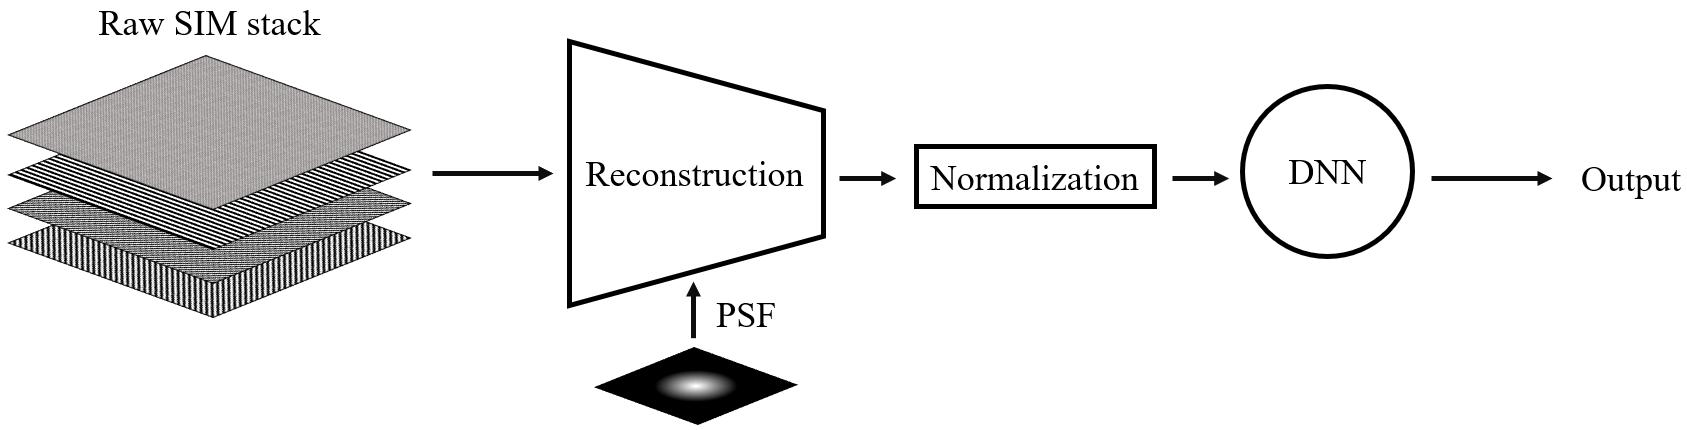
\includegraphics[width=0.48\textwidth]{images/system_block_diagram.png}
    \caption{High-level block diagram of the complete 4-image SR-SIM reconstruction system.}
    \label{fig:system_block_diagram}
\end{figure}

\subsection{Evaluation metrics}
To compare the performance of the DNNs, they were evaluated on three simulated SIM test images (created as explained in the second paragraph of section \ref{sec:Dataset}), two of which were taken from biological cell structures and one that was derived from a printer test image. Test image 1 contains Filamentous actin and microtubules in mouse fibroblasts \cite{test_image_1_ref} and test image 2 is a image of microtubules in a Drosophila S2 cell \cite{test_image_2_ref}. While not having any biological affiliation, test image 3 contains interesting isolated high-frequency structures like the one seen in figure \ref{fig:circle_comp} that proved useful to assess the systems super-resolution performance.

To gain a representative insight on the model's performance a total of three metrics were used. The first one was the structural similarity index measure (SSIM) \cite{ssim_article} given by
$$\operatorname{SSIM}(x, y) = S_{1}(x, y)S_{2}(x, y)$$
with
\begin{align*} 
    S_{1}(x, y) =& \frac{2\bar{x}\bar{y} + c_{1}}{ \bar{x}^{2} + \bar{y}^{2} + c_{1}}\\ S_{2}(x, y) =& \frac{2s_{x, y} + c_{2}}{s_{x}^{2} + s_{y}^{2} + c_{2}}
\end{align*}
where $\bar{x}$, $\bar{y}$, $s_{x}^{2}$, $s_{y}^{2}$ and $s_{x, y}$ respectively represent the local mean, variance and covarianve of the two images $x$ and $y$. The second was the peak signal to noise ratio (PSNR) \cite{PSNR_paper} defined as
$$\operatorname{PSNR}(x, y)=20\log_{10}\left(\frac{\operatorname{max}(y)}{\sqrt{\overline{(x-y)^2}}}\right).$$
Finally, the Fourier ring correlation (FRC) \cite{FRC_paper} was used, which is given by
$$\operatorname{FRC}(x,y,R)=\frac{\sum_{i\in R}X(r_i)\cdot Y(r_i)^*}{\sqrt{\left(\sum_{i\in R}|X(r_i)|^2\right)\cdot \left(\sum_{i\in R}|Y(r_i)|^2\right)}}$$
where $X$ and $Y$ are the Fourier transforms of the images $x$ and $y$. The FRC is a metric that is often used to compare the resolution of images. It calculates the correlation between the Fourier transforms of the two images within the ring of a given width and radius, creating a graph that represents the similarity of two images as the observation resolution is increased. To gain a single-number representation of the FRC the Fourier ring correlation energy (FRCE) was computed as
$$\operatorname{FRCE}(x,y)=\int_{0}^\pi\operatorname{FRC}(x,y,R)\,dR$$

\smallskip
\section{Results}
\subsection{DNN Training}
\label{sec:dnn_training}

\begin{figure}[h]
    \centering
    \begin{subfigure}[b]{0.157\textwidth}
        \centering
        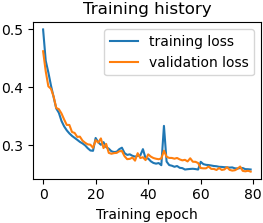
\includegraphics[width=\textwidth]{images/train_hist_snrMIX.png}
        \caption{snrMIX}
        \label{fig:train_hist_snrMIX}
    \end{subfigure}
    \begin{subfigure}[b]{0.157\textwidth}
        \centering
        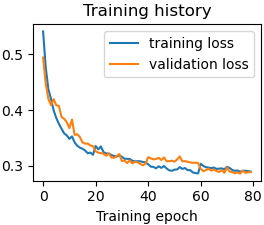
\includegraphics[width=\textwidth]{images/train_hist_snrMIX2.png}
        \caption{snrMIX2}
        \label{fig:train_hist_snrMIX2}
    \end{subfigure}
    \begin{subfigure}[b]{0.162\textwidth}
        \centering
        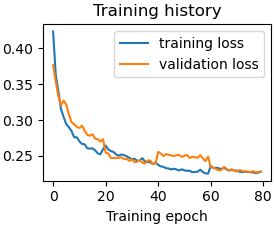
\includegraphics[width=\textwidth]{images/train_hist_snrMIX3.png}
        \caption{snrMIX3}
        \label{fig:train_hist_snrMIX3}
    \end{subfigure}
    \caption{Training history of the three main DNNs.}
    \label{fig:train_curves}
\end{figure}

Since one of the main goals of this project was to improve the noise resistance of the existing 4-image algorithm, three structurally similar DNNs have been trained on different dataset combinations, each one containing the same Ground-Truth images but input images that have been reconstructed with different signal-to-noise ratio (SNR) levels. The first dataset, called \textit{snrMIX}, consists of an equal amount of images with SNRs $[5,10,20,35]$ in dB. The idea behind this combination was to provide varying levels of artefacts with the first three SNRs, but also provide a nearly perfect image with the 35dB one, so that a nearly noiseless input would not be artificially distorted. The second one, called \textit{snrMIX2} contains the SNRs $[5,10,15,20]$, where the 35dB inputs were replaced by images with an SNR of 15dB to create a uniform distribution of SNRs between 5dB and 20dB. The last one, called \textit{snrMIX3} is only made up of the two SNRs $[15,20]$, which has been chosen to analyse the effect of missing low SNRs during training on the final performance. 

All three models have been trained for 80 epochs, while switching between the two halves of the dataset every 20 epochs as explained in section \ref{sec:Dataset}. The resulting training curves presented in figure \ref{fig:train_curves}, show that no overfitting occurred during the training process as both the training and validation loss decrease at roughly the same rate. 

\subsection{Test Images}

As mentioned before, the DNNs have been tested on three different test images. An overview of the numerical results is given in table \ref{tab:results_comparison}. It shows the SSIM, PSNR and FRCE values for the DNN input, which in our case is the 4-image SR-SIM reconstruction, the widefield and the DNN outputs, when compared to the ground-truth of the corresponding test image. Each of the three test images was created 4 times with varying SNRs to study the noise resistance of the DNNs. Looking at the table, it can be noted that no matter the SNR value of the test image used, all three networks deliver greatly improved results compared to both the widefield and the reconstruction. Furthermore, for test images 1 and 2, the reconstruction performs even worse than the widefield at low SNR values.

% test images: 4=1, 2=2, 3=3
\begin{table}[h]
    \tabcolsep=0.11cm
    \resizebox{\columnwidth}{!}{
    \begin{tabular}{l|l|l|l}
    Image 1   & \multicolumn{1}{c|}{SSIM} & \multicolumn{1}{c|}{PSNR} & \multicolumn{1}{c}{FRCE} \\ \hline
    Reconstr. & 0.24 / 0.37 / 0.53 / 0.65                          & 10.39 / 12.56 / 15.41 / 17.80                      & 0.16 / 0.24 / 0.31 / 0.36                         \\
    Widefield      & 0.30 / 0.45 / 0.59 / 0.67                          & 11.76 / 14.42 / 16.97 / 19.03                      & 0.22 / 0.27 / 0.30 / 0.32                         \\
    snrMIX         & 0.78 / 0.81 / 0.85 / 0.89                          & 20.22 / 20.32 / 21.37 / 24.19                      & 0.41 / 0.44 / 0.46 / 0.48                         \\
    snrMIX2        & 0.79 / 0.84 / 0.87 / 0.88                          & 20.09 / 20.61 / 21.99 / 22.34                      & 0.41 / 0.44 / 0.46 / 0.48                         \\
    snrMIX3        & 0.78 / 0.85 / 0.88 / 0.90                          & 19.98 / 21.33 / 21.80 / 22.69                      & 0.38 / 0.43 / 0.46 / 0.48                        
    \end{tabular}
    }
    \newline
    \vspace*{0.2 cm}
    \newline
    \tabcolsep=0.11cm
    \resizebox{\columnwidth}{!}{
    \begin{tabular}{l|l|l|l}
    Image 2   & \multicolumn{1}{c|}{SSIM} & \multicolumn{1}{c|}{PSNR}     & \multicolumn{1}{c}{FRCE}  \\ \hline
    Reconstr. & 0.31 / 0.45 / 0.58 / 0.68 & 12.37 / 14.56 / 17.31 / 19.98 & 0.20 / 0.28 / 0.34 / 0.39 \\
    Widefield & 0.39 / 0.52 / 0.63 / 0.70 & 14.08 / 16.71 / 18.80 / 20.34 & 0.24 / 0.29 / 0.31 / 0.32 \\
    snrMIX    & 0.85 / 0.89 / 0.93 / 0.95 & 21.52 / 22.67 / 24.56 / 26.38 & 0.38 / 0.43 / 0.47 / 0.51 \\
    snrMIX2   & 0.89 / 0.91 / 0.89 / 0.88 & 22.60 / 22.73 / 23.07 / 23.74 & 0.39 / 0.43 / 0.47 / 0.50 \\
    snrMIX3   & 0.84 / 0.90 / 0.90 / 0.94 & 20.98 / 21.50 / 22.78 / 25.45 & 0.37 / 0.42 / 0.47 / 0.50
    \end{tabular}
    }
    \newline
    \vspace*{0.2 cm}
    \newline
    \tabcolsep=0.11cm
    \resizebox{\columnwidth}{!}{
    \begin{tabular}{l|l|l|l}
    Image 3   & \multicolumn{1}{c|}{SSIM} & \multicolumn{1}{c|}{PSNR}     & \multicolumn{1}{c}{FRCE}  \\ \hline
    Reconstr. & 0.27 / 0.36 / 0.42 / 0.44 & 10.97 / 12.26 / 13.31 / 13.82 & 0.23 / 0.31 / 0.36 / 0.39 \\
    Widefield & 0.29 / 0.31 / 0.30 / 0.28 & 11.42 / 11.52 / 11.47 / 11.38 & 0.28 / 0.32 / 0.34 / 0.36 \\
    snrMIX    & 0.88 / 0.93 / 0.94 / 0.90 & 18.99 / 21.52 / 21.45 / 19.67 & 0.47 / 0.53 / 0.55 / 0.56 \\
    snrMIX2   & 0.83 / 0.84 / 0.91 / 0.90 & 16.43 / 16.52 / 19.84 / 19.77 & 0.49 / 0.52 / 0.53 / 0.52 \\
    snrMIX3   & 0.84 / 0.89 / 0.89 / 0.88 & 16.93 / 17.38 / 18.46 / 19.01 & 0.48 / 0.53 / 0.53 / 0.51
    \end{tabular}
    }
    \caption{Comparison of the 4-image SR-SIM reconstruction ("Reconstr."), Widefield, \textit{snrMIX}-, \textit{snrMIX2}- and \textit{snrMIX3} model with the ground-truth. The results are obtained by using test images 1, 2 and 3 with SNR values (5dB / 10dB / 15dB / 20dB) as the input image to the system.}
    \label{tab:results_comparison}
\end{table}

Figure \ref{fig:test_img_4_model_comp_snr10} shows a visual comparison in a zoomed region of test image 1. The reconstruction and the widefield image have been generated with an SNR of 10dB and the net outputs are the direct result of providing this reconstruction as the input image to the DNN. The visible region has a size of $150 \times 150$ pixels (4.8$\mu$m$^2$) and the main fibres that can be seen have a simulated diameter of around 3-4 pixels ($\sim$100nm). In the ground-truth, in the bottom left part of the image, two parallel fibers can be seen close together but not quite overlapping. In the widefield image however, the two fibers cannot be distinguished from each other at their closest position, showcasing the loss in resolution. While barely visible, the fibers can still be distinguished in all three DNN outputs.

\begin{figure}[h]
    \centering
    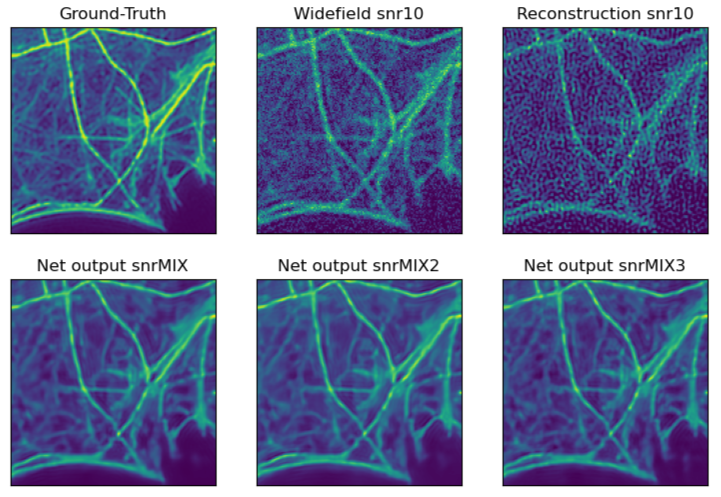
\includegraphics[width=0.48\textwidth]{images/test_img_4_model_comp_snr10.png}
    \caption{Visual comparison of widefield, reconstruction and the three DNN outputs in a zoomed region from test image 1 with SNR=10dB.}
    \label{fig:test_img_4_model_comp_snr10}
\end{figure}
\begin{figure}[h]
    \centering
    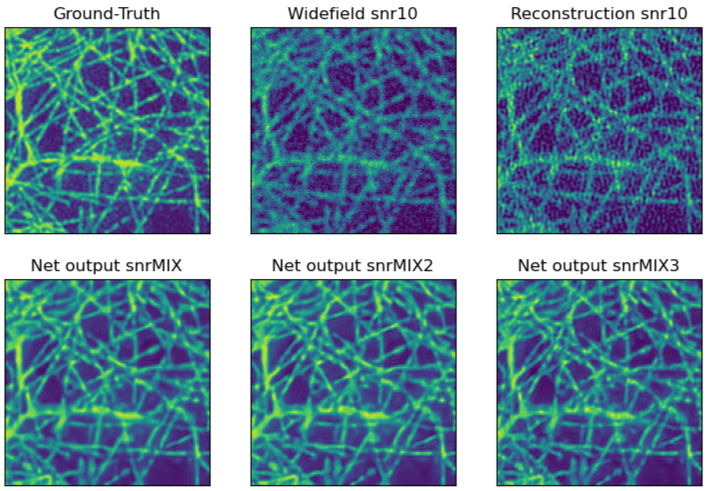
\includegraphics[width=0.48\textwidth]{images/test_img_2_model_comp_snr10.png}
    \caption{Visual comparison of widefield, reconstruction and the three DNN outputs in a zoomed region from test image 2 with SNR=10dB.}
    \label{fig:test_img_2_model_comp_snr10}
\end{figure}

In figure \ref{fig:test_img_2_model_comp_snr10} a zoomed region of test image 2 can be seen. The visible window is of size $150 \times 150$ pixels (4.8$\mu$m$^2$) and the fibres have a diameter of around 3-4 pixels ($\sim$100nm). In the middle and top left of this window, the ground-truth shows thin parallel lines that are only separated by around 2-3 pixels ($\sim$85nm or around half the diffraction limit). In the widefield and the reconstruction these lines look as though they are merged together and also in the DNN outputs they are hard to distinguish. Still in all three output images there is at least an indication of the two lines.

\begin{figure}[h!]
    \centering
    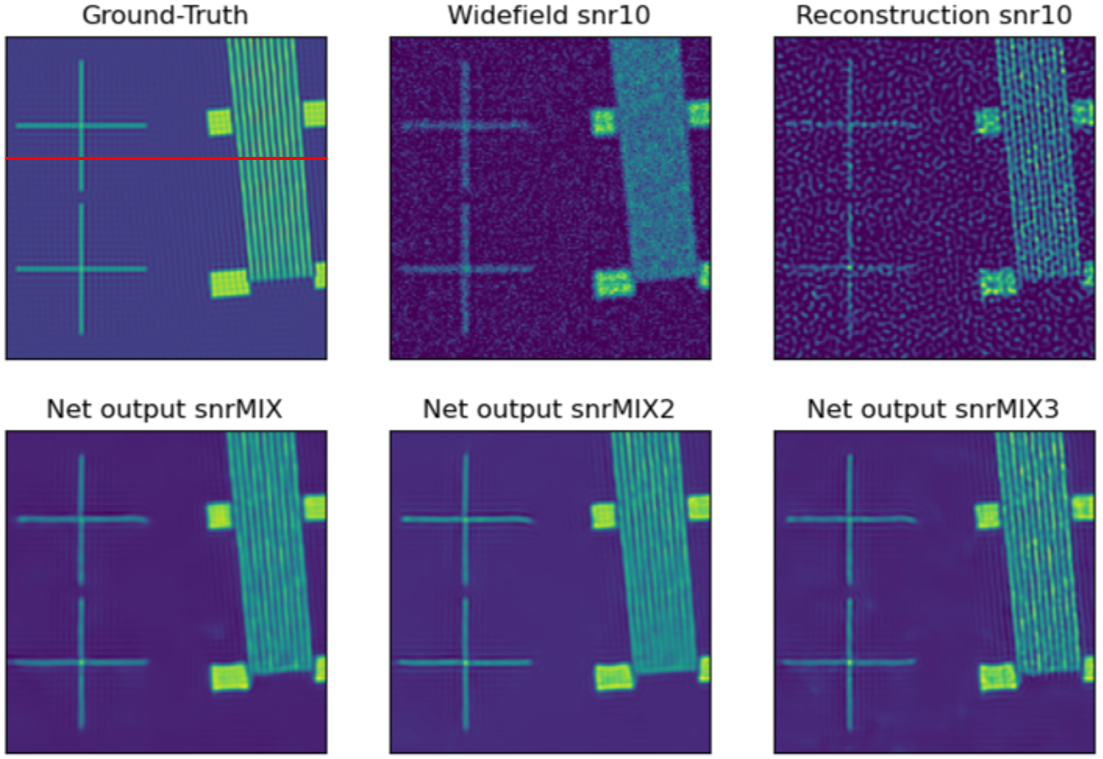
\includegraphics[width=0.48\textwidth]{images/test_img_3_model_comp_snr10_cross_line.png}
    \caption{Visual comparison of widefield, reconstruction and the three DNN outputs in a zoomed region (lines) from test image 3 with SNR=10dB.}
    \label{fig:test_img_3_model_comp_snr10_cross}
\end{figure}
\begin{figure}[h!]
    \centering
    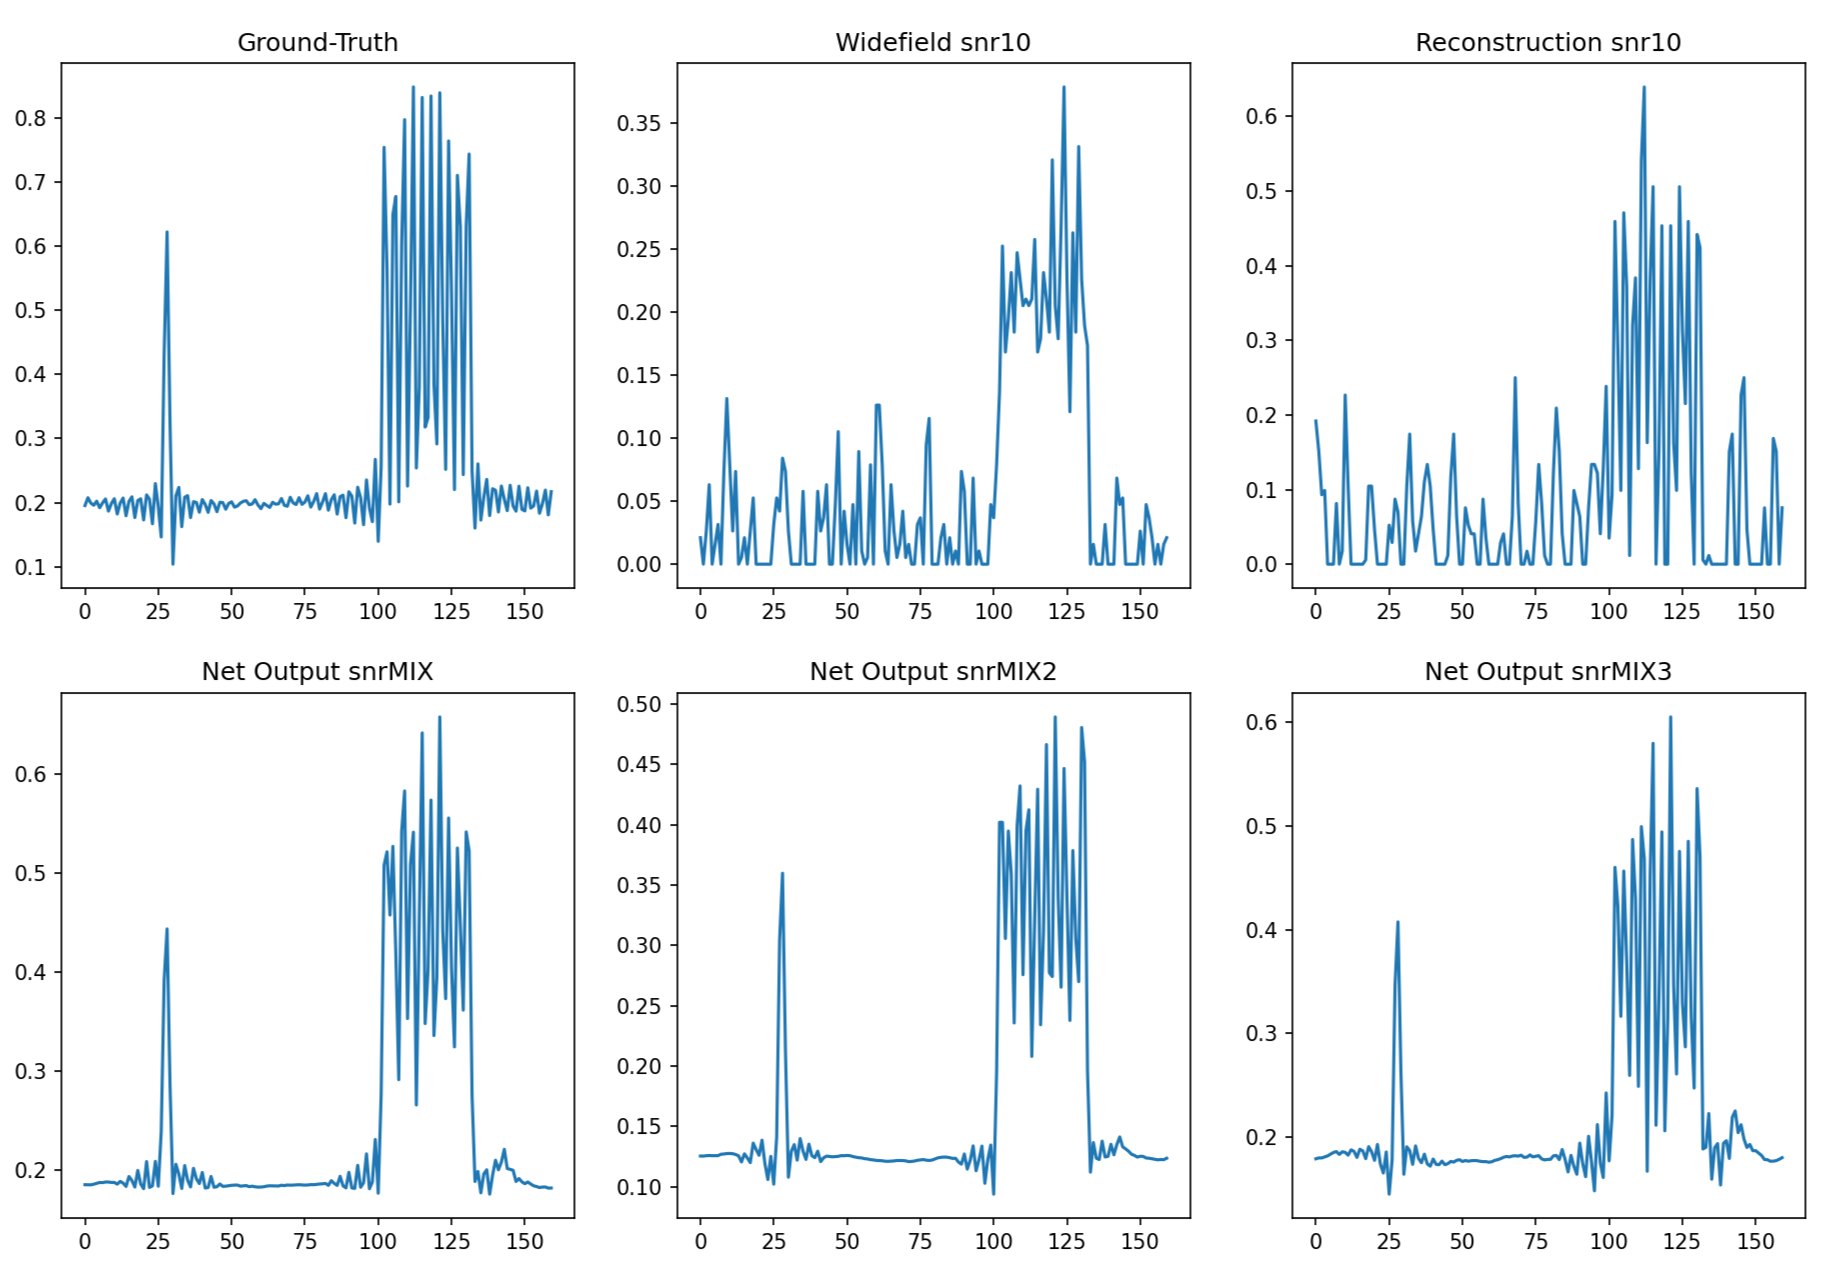
\includegraphics[width=0.48\textwidth]{images/test_img_3_model_comp_snr10_cross_cut.png}
    \caption{Intensity profile of a horizontal cut (indicated by the red line) through the region visible in figure \ref{fig:test_img_3_model_comp_snr10_cross}.}
    \label{fig:test_img_3_model_comp_snr10_cross_cut}
\end{figure}

As mentioned before, especially test image 3 contains some interesting features that serve to visually compare the systems super-resolution performance. Figure \ref{fig:test_img_3_model_comp_snr10_cross} shows one of these features, containing a thin cross with a line width of around 2 pixels ($\sim$64nm) on the left and multiple thin parallel lines of around 2-3 pixels ($\sim$85nm) in width and separation on the right. The visible window is of size $129 \times 129$ pixels (4.128$\mu$m$^2$). It has been chosen smaller than the other widows so that the very thin lines can be distinguished more easily. By looking at this figure it can be seen that the parallel thin lines are completely lost in the widefield image and could not be distinguished from a large flat surface of uniform illumination. In the reconstruction the lines are barely visible but heavily distorted. Finally, in all DNN outputs the lines are visible and the artefacts have completely been removed. The proper separation of the lines is best provided by \textit{snrMIX3}.

\begin{figure}[h]
    \centering
    \vspace{0.47cm}
    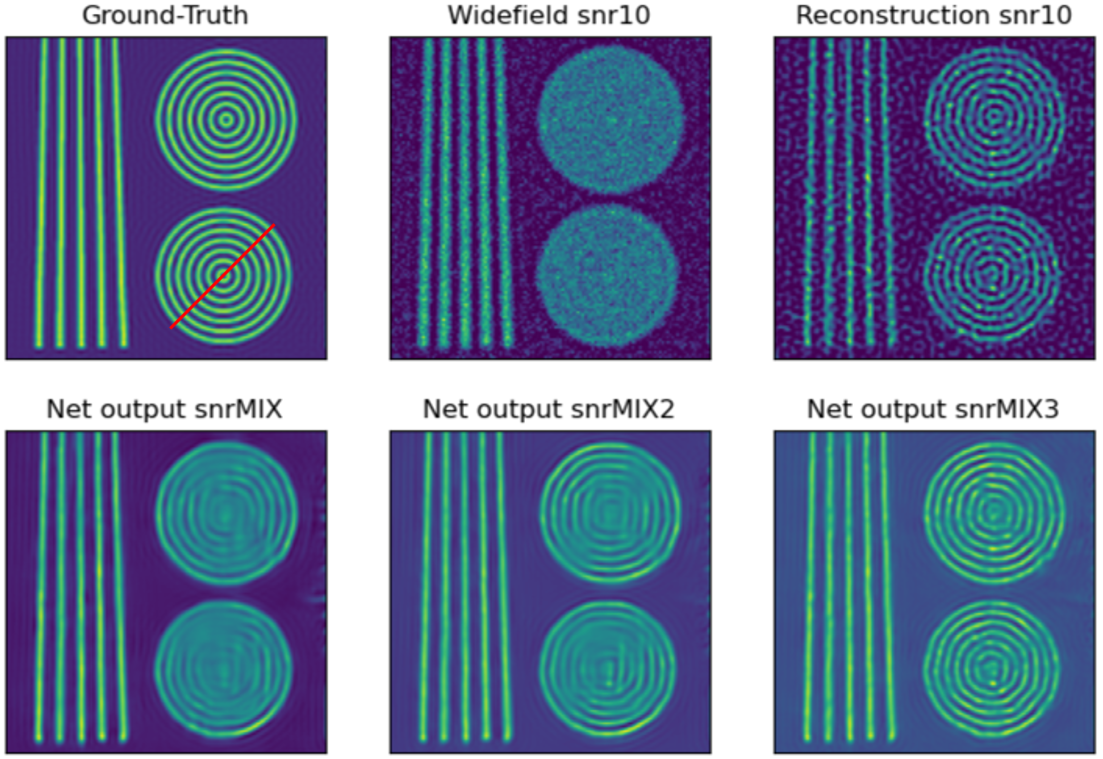
\includegraphics[width=0.48\textwidth]{images/test_img_3_model_comp_snr10_circle_line.png}
    \caption{Visual comparison of widefield, reconstruction and the three DNN outputs in a zoomed region (circles) from test image 3 with SNR=10dB.}
    \label{fig:test_img_3_model_comp_snr10_circle}
\end{figure}
\begin{figure}[h]
    \centering
    \vspace{0.2cm}
    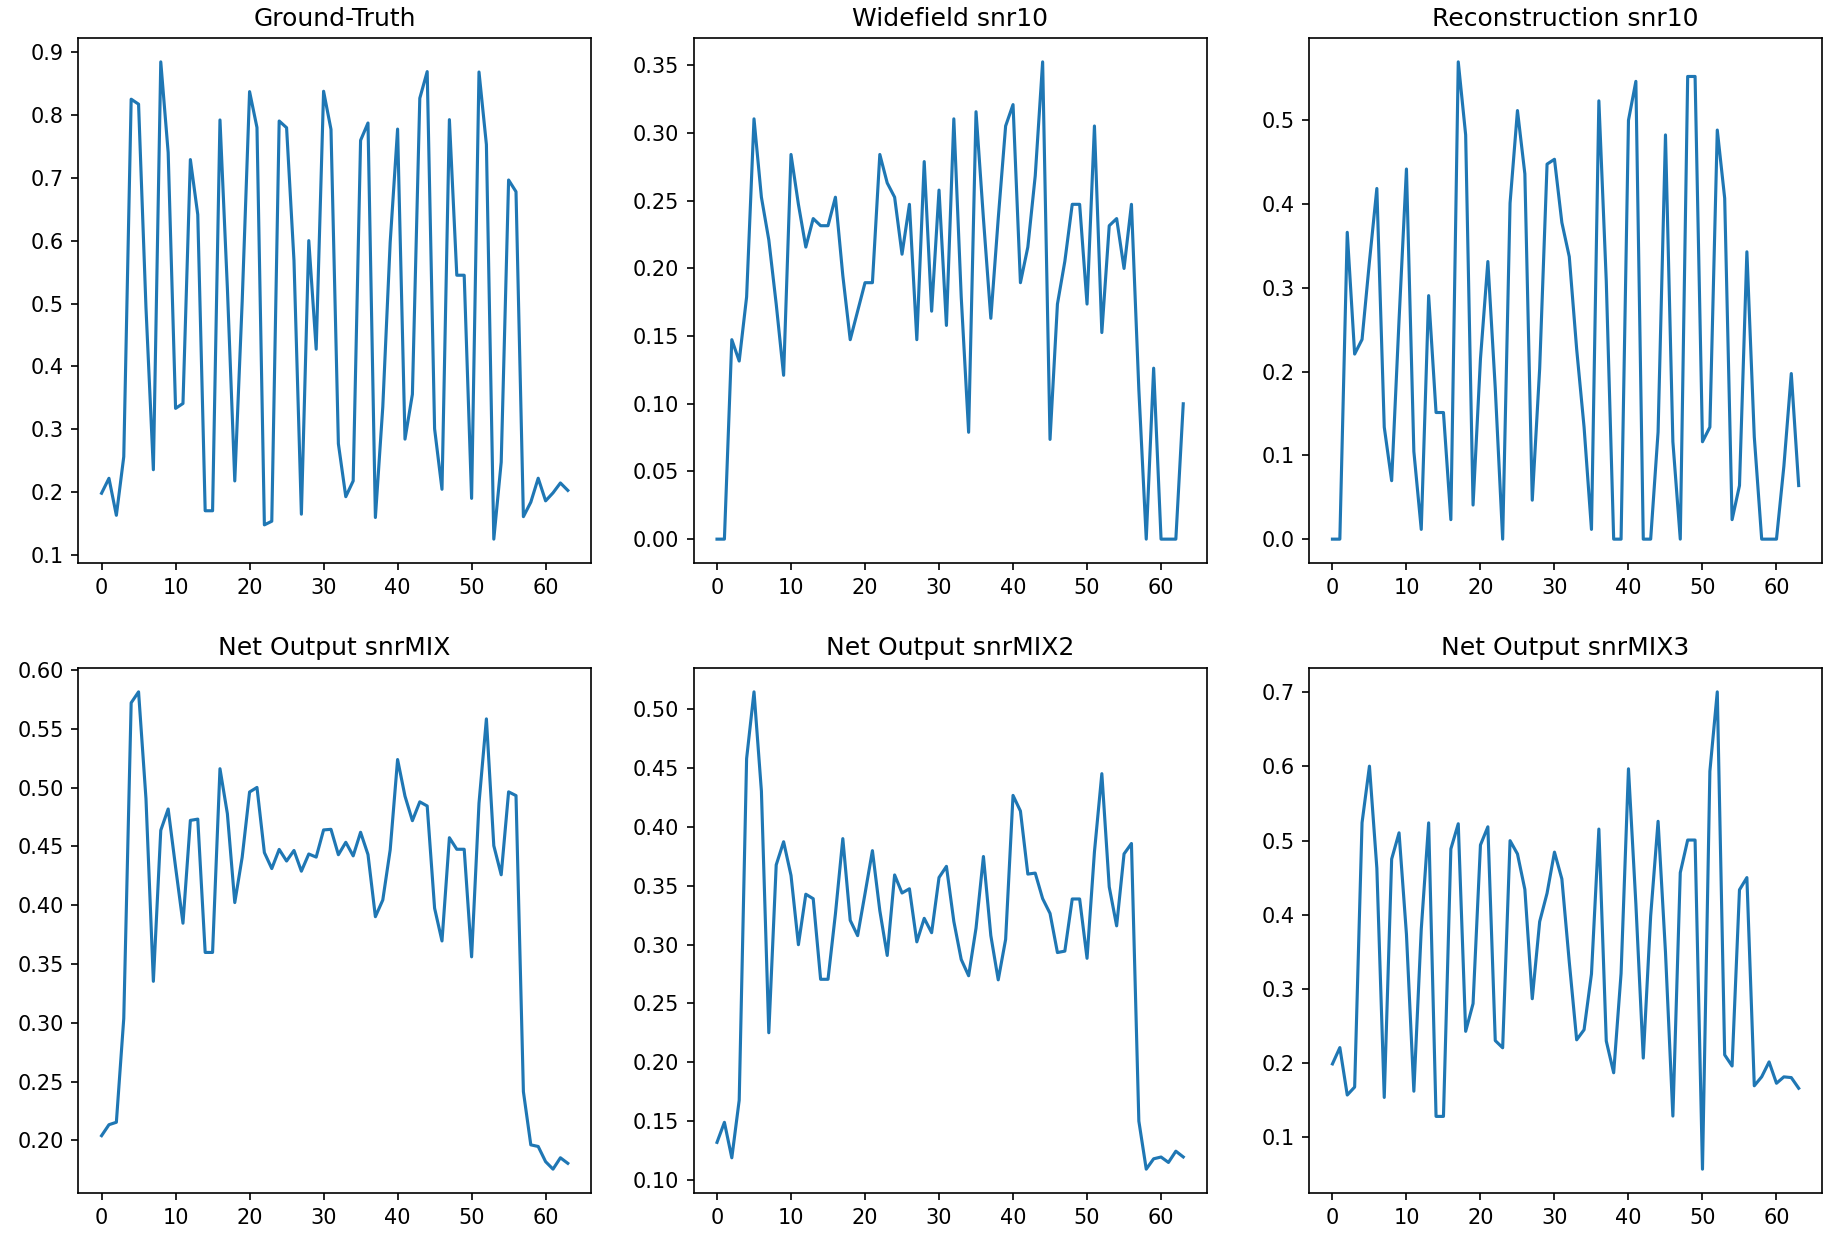
\includegraphics[width=0.48\textwidth]{images/test_img_3_model_comp_snr10_circle_cut.png}
    \caption{Intensity profile of a diagonal cut at 45$^\circ$ (indicated by the red line) through the circles visible in figure \ref{fig:test_img_3_model_comp_snr10_circle}.}
    \label{fig:test_img_3_model_comp_snr10_cirlce_cut}
\end{figure}

The second feature of test image 3 is shown in figure \ref{fig:test_img_3_model_comp_snr10_circle}. It contains thin nested circles with a width and separation of around 2-3 pixels ($\sim$85nm). This circular pattern is especially interesting, since as we saw in the choice of DNN structure, it demonstrates the systems super-resolution capability for all possible orientations. As in the previous parallel lines, the thin circles cannot be distinguished from a solid disc in the widefield image. In the reconstruction, the circles are clearly visible but heavily distorted by artefacts. While the circles are generally visible in all net outputs, the \textit{snrMIX3} network provides the best result in terms of separating the individual circles at all orientations.

In order to analyse the DNNs performance for these two defining features, intensity profiles have been generated, representing the pixel values along a given line through the images. Figure \ref{fig:test_img_3_model_comp_snr10_cross_cut} shows the intensity profile on a horizontal line through the upper part of the visible window in figure \ref{fig:test_img_3_model_comp_snr10_cross}. On the ground-truth profile, the thin vertical line of the cross can be seen as a spike on the left and the thin parallel lines are represented as an oscillating block on the right. In the widefield image, the spike of the cross is completely missing on this particular line and as observed before, the thin parallel lines cannot be distinguished from each other. There is also a lot of noise in both the background and the object. In the reconstruction, the line of the cross is also missing on this line, but the parallel lines can still be recognized. Similar to the widefield profile, a lot of noise (artefacts) are present everywhere. All the DNN outputs clearly show the vertical line of the cross as well as the parallel lines and at the same time, the noise has been reduced considerably. The \textit{snrMIX3} network provides the largest oscillation amplitude for the parallel lines.

Figure \ref{fig:test_img_3_model_comp_snr10_cirlce_cut} shows the intensity profile of a line crossing the bottom circular pattern of figure \ref{fig:test_img_3_model_comp_snr10_circle} at a 45$^\circ$ angle. In the ground-truth profile, the circular pattern can be distinguished by the heavily oscillating line. In the widefield profile, the line is oscillating randomly with a small amplitude due to noise and in the reconstruction profile there is a clear oscillation that is perturbed by the present artefacts. Looking at the output of \textit{snrMIX} and \textit{snrMIX2}, there is only a slight oscillation on this specific line angle. The output of \textit{snrMIX3} however, provides a very clear oscillation pattern.

\begin{figure}[h]
    \centering
    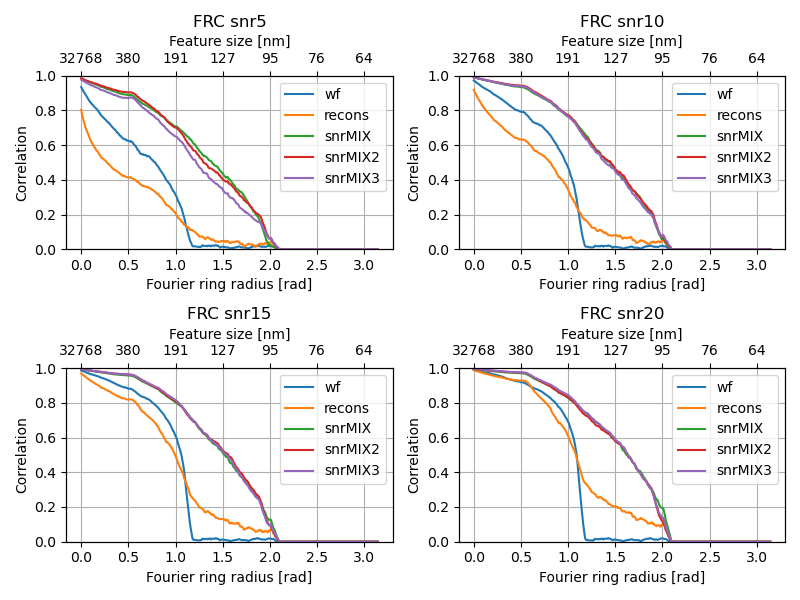
\includegraphics[width=0.48\textwidth]{images/test_img_4_comp_frc.png}
    \caption{FRC curves of test image 1 for different SNR values.}
    \label{fig:test_img_4_comp_frc}
\end{figure}

While the visual comparison can give a good indication of the DNNs performance, a numerical approach has also been implemented. As the SSIM and the PSNR only deliver one number for a given image, it can be difficult to correctly interpret the results. For this reason, all three test images have been analysed using the FRC, which is able to represent the similarity of two images as a function of the resolution. Using this metric allows for a more detailed analysis of the super-resolution performance.

Figures \ref{fig:test_img_4_comp_frc}, \ref{fig:test_img_2_comp_frc} and \ref{fig:test_img_3_comp_frc} show the FRC curves of the widefield and the 4-image SR-SIM reconstruction as well as the curves of the three trained models for the three test images with varying SNR values. The bottom x-axis represents the spatial frequency, while the top x-axis represents the corresponding size of the structures that can be represented at that frequency. First of all, it can be noted that all curves stay at zero below a feature size of around 90nm, which approximately corresponds to half the simulated diffraction limit of 174.3nm. This makes sense, since the Fourier transform of the ground-truth image was masked accordingly and is zero outside this range. Another observation that applies to all test images, is the sharp drop in the FRC value of the widefield image at the diffraction limit of around 174.3nm, representing the limited resolution capability in normal widefield microscopy.

\begin{figure}[h]
    \centering
    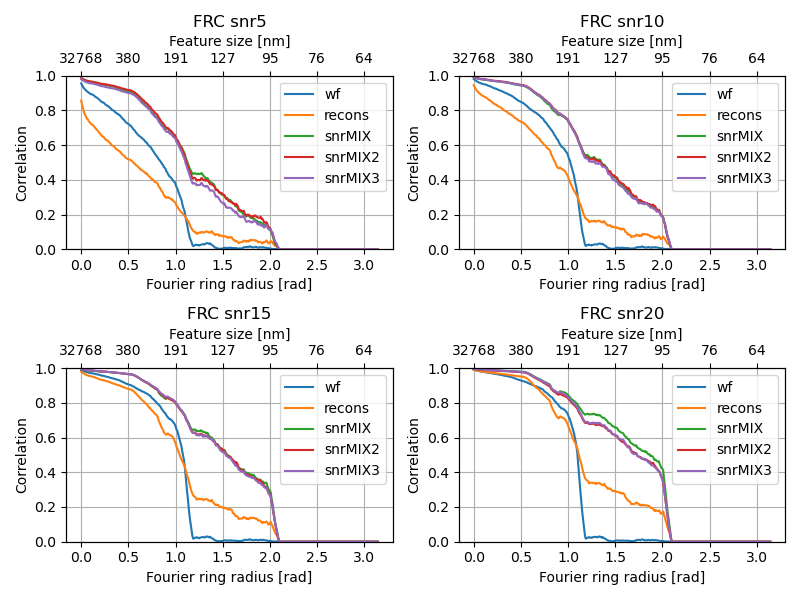
\includegraphics[width=0.48\textwidth]{images/test_img_2_comp_frc.png}
    \caption{FRC curves of test image 2 for different SNR values.}
    \label{fig:test_img_2_comp_frc}
\end{figure}

Looking at figure \ref{fig:test_img_4_comp_frc}, which shows the FRC curves of test image 1, it can be observed that the FRC values of all DNN outputs are similar and decrease much slower that the FRC values of both the widefield and the reconstruction images. There is also no sharp drop at the diffraction limit in any of the network outputs, rather they steadily decrease up to half the diffraction limit. Furthermore, especially at lower SNR values (5dB and 10dB) the reconstruction image has a lower FRC value than the widefield up until the diffraction limit.

\begin{figure}[h]
    \centering
    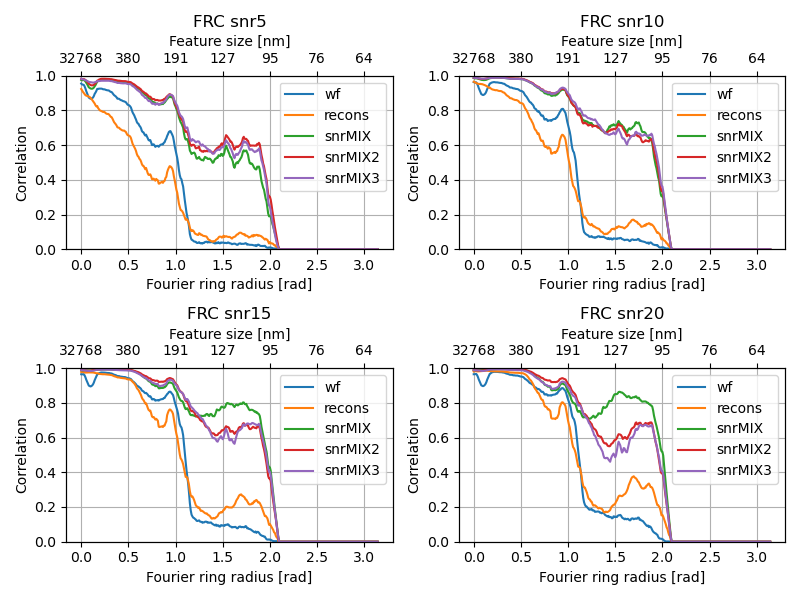
\includegraphics[width=0.48\textwidth]{images/test_img_3_comp_frc.png}
    \caption{FRC curves of test image 3 for different SNR values.}
    \label{fig:test_img_3_comp_frc}
\end{figure}

In figure \ref{fig:test_img_2_comp_frc}, which shows the FRC curves for test image 2, the FRC curves of the three DNNs are again similar, but show a slight drop at the diffraction limit, especially at lower SNR values. Overall the FRC decrease is not as smooth as for the first test image, but all DNN outputs still provide much better results than both the widefield and reconstruction images. Again, at low SNR values, the reconstruction seems to perform worse than the widefield up until the diffraction limit.

Finally, figure \ref{fig:test_img_3_comp_frc} shows the FRC curves for test image 3. The curves for this test image look quite different than those seen for test images 1 and 2. In general, the curves provided by this test image are not as smooth as the others. There are several spikes and not all curves are decreasing monotonously. Especially at higher SNR values, the reconstruction and net output curves start increasing again below the diffraction limit. Additionally, in contrast to the other two test images, the net output curves are not similar for all SNR values. At an SNR of 10dB and 20dB, the \textit{snrMIX} curve stays higher than the others below the diffraction limit.

\section{Discussion}
Overall, looking at the provided results, it could be established that the proposed DNN is capable of correcting a 4-image SR-SIM reconstruction image and provide a clean super-resolved image at twice the resolution compared to a widefield image. Numerically, looking at table \ref{tab:results_comparison}, the three proposed networks that have been trained on different combinations of SNR values present in the dataset show no significant preference for any one network, with exception of the PSNR values obtained for test image 3. Considering the FRC curves (figures \ref{fig:test_img_4_comp_frc}, \ref{fig:test_img_2_comp_frc} and \ref{fig:test_img_3_comp_frc}), the only difference between the three version can be seen in test image 3 and only for the SNR values 15dB and 20dB, where the \textit{snrMIX} network performs better than the other two at high frequencies. However, when looking at the visual comparison made in figures \ref{fig:test_img_3_model_comp_snr10_cross}, \ref{fig:test_img_3_model_comp_snr10_cross_cut}, \ref{fig:test_img_3_model_comp_snr10_circle} and \ref{fig:test_img_3_model_comp_snr10_cirlce_cut}, the \textit{snrMIX3} network seems to provide better results as both the thin lines and circles can be distinguished more easily than in the other net outputs. This is mostly due to the fact that the \textit{snrMIX3} doesn't smoothen the image as much as the other networks, which enables it to produce clearer results in high frequency areas like the ones explored, but also has the effect of introducing more variation in the background areas of the image as can be seen in figure \ref{fig:test_img_3_model_comp_snr10_cross}. Taking into account that the main objective of the DNN is to enable super-resolution with clearly visible high frequency features, the background does not really play an important role as long as it is clearly separable from the main features. Additionally, as seen for the test images 1 and 2 that contain actual biological data, the background is usually not as even as in the "artificial" test image 3, meaning that some variation in the background already exists by default.

From the gathered observation, it would seem as the \textit{snrMIX3} network provides the most preferable results, especially at low SNR values. This conclusion is rather unexpected, since \textit{snrMIX3} was the only DNN that hasn't been trained on any low-SNR training images. In fact, as mentioned in section \ref{sec:dnn_training}, this network was only trained on images with SNRs of 15dB and 20dB, while \textit{snrMIX} was also trained on 5dB and \textit{snrMIX2} on 5dB and 10dB SNR values. One possible explanation for this unintuitive behaviour could be the incredibly large amount of artefacts introduced by the reconstruction algorithm at an SNR of 5dB, which might make it impossible for the implemented network architecture to correctly recreate high frequency structures and thus simply learns to smoothen the image in order to obtain a better comparison score. Since the \textit{snrMIX3} network was never exposed to such low SNR values, it would just apply the same strategy used for high SNR images, providing observably better results.

At this point it should also be mentioned that the chosen RCAN network depth was considerably shallower than the originally proposed RCAN structure that consisted of 10 residual groups, each one containing 20 residual channel attention blocks \cite{zhang2018rcan} compared to the 3 groups and 5 blocks used in this project. The limiting factor in terms of depth was the available GPU memory, which wouldn't allow for the backward-pass calculation of a deeper network. It could be argued that a deeper network would be able to better correct such low SNR values when being trained correctly, however training a much deeper network with considerably more trainable parameters generally makes the training process more difficult and ultimately results in a longer execution time.

\section{Conclusion}
This project has shown that using a 4-image SR-SIM reconstruction algorithm together with a DNN to correct artefacts, provides a reliable, fast and noise resistant alternative to current SR-SIM reconstruction techniques when using simulated SIM images. Concerning the DNN, the best overall results were obtained by not providing any low-SNR images during training, because this promoted smoothing of the output image, causing the 
deterioration of certain high frequency features for low-SNR input images. While the presented method in its current state cannot be directly applied to real SIM images, as the reconstruction algorithm only works with an ideal PSF, the obtained results demonstrated the possibility of such a system, which could easily be adapted to real SIM images once an improved reconstruction algorithm has been developed.

\newpage
\bibliographystyle{IEEEtran}
\bibliography{IEEEabrv,biblio_traps_dynamics}

\newpage
\section{Appendix}
\subsection{Supplementary figures}
\begin{figure}[h!]
    \centering
    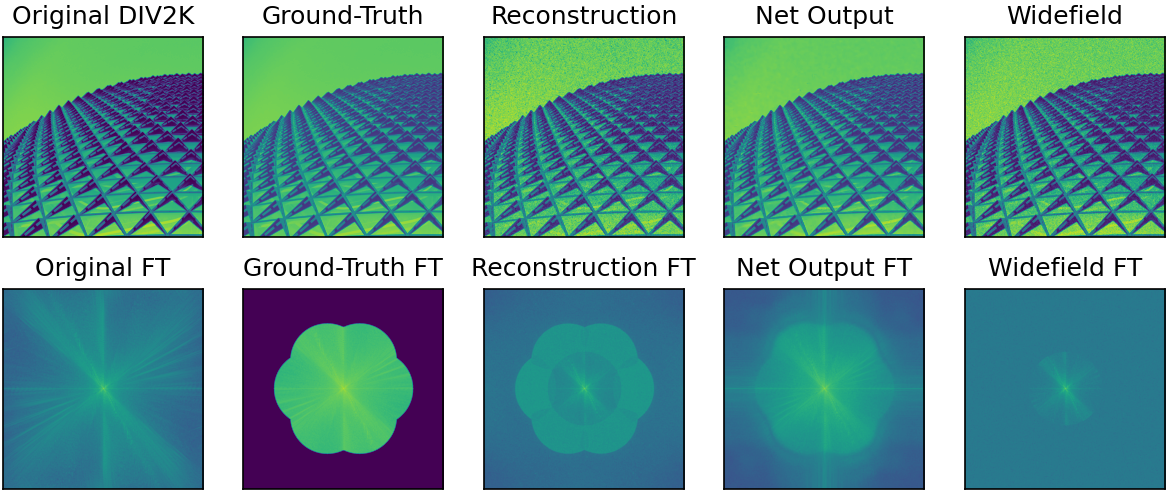
\includegraphics[width=0.48\textwidth]{images/images_and_FTs_extended.png}
    \caption{Comparison of the ground-truth, net input (reconstruction), net output and widefield in the space and frequency domain for a sample training image at SNR=10dB.}
    \label{fig:images_and_FTs_output}
\end{figure}
\begin{figure}[h!]
    \centering
    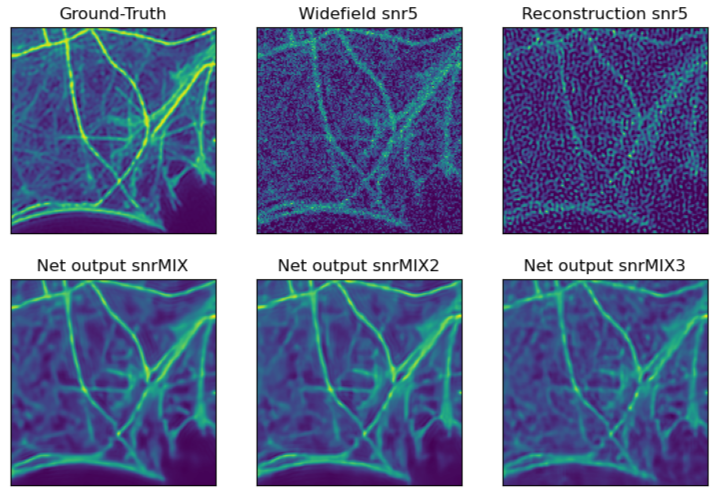
\includegraphics[width=0.48\textwidth]{images/test_img_4_model_comp_snr5.png}
    \caption{Visual comparison of widefield, reconstruction and the three DNN outputs in a zoomed region from test image 1 with SNR=5dB.}
    \label{fig:test_img_4_model_comp_snr5}
\end{figure}
\begin{figure}[h!]
    \centering
    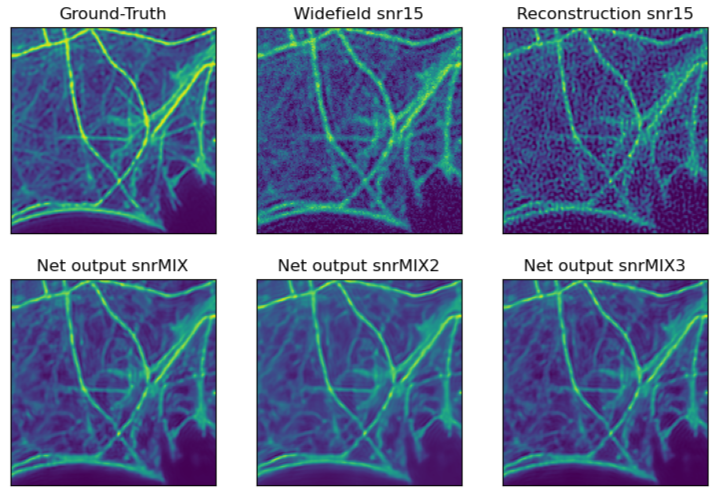
\includegraphics[width=0.48\textwidth]{images/test_img_4_model_comp_snr15.png}
    \caption{Visual comparison of widefield, reconstruction and the three DNN outputs in a zoomed region from test image 1 with SNR=15dB.}
    \label{fig:test_img_4_model_comp_snr15}
\end{figure}
\begin{figure}[h!]
    \centering
    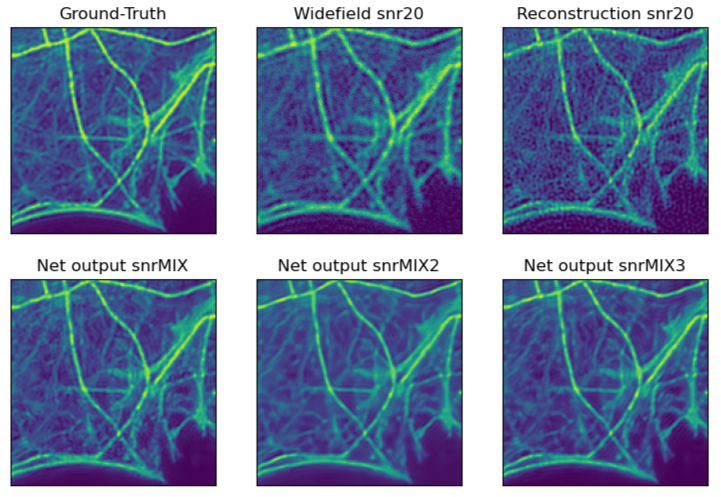
\includegraphics[width=0.48\textwidth]{images/test_img_4_model_comp_snr20.png}
    \caption{Visual comparison of widefield, reconstruction and the three DNN outputs in a zoomed region from test image 1 with SNR=20dB.}
    \label{fig:test_img_4_model_comp_snr29}
\end{figure}
\begin{figure}[h!]
    \centering
    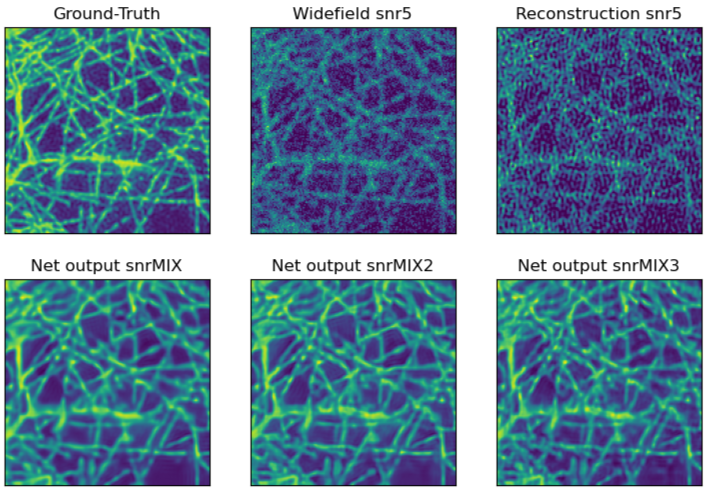
\includegraphics[width=0.48\textwidth]{images/test_img_2_model_comp_snr5.png}
    \caption{Visual comparison of widefield, reconstruction and the three DNN outputs in a zoomed region from test image 2 with SNR=5dB.}
    \label{fig:test_img_2_model_comp_snr5}
\end{figure}
\begin{figure}[h!]
    \centering
    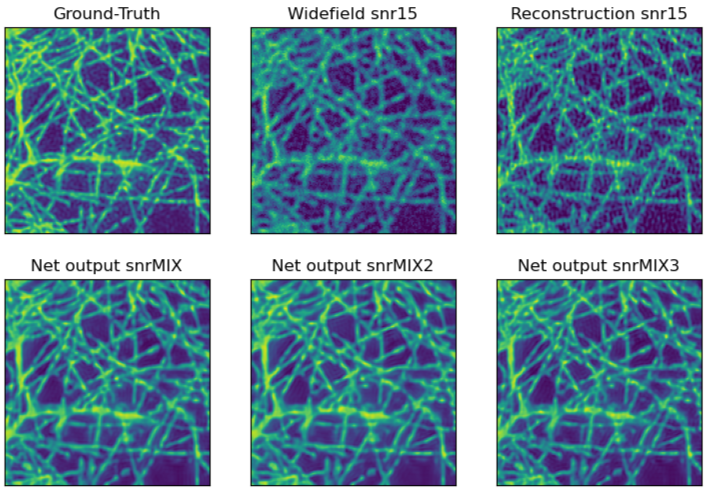
\includegraphics[width=0.48\textwidth]{images/test_img_2_model_comp_snr15.png}
    \caption{Visual comparison of widefield, reconstruction and the three DNN outputs in a zoomed region from test image 2 with SNR=15dB.}
    \label{fig:test_img_2_model_comp_snr15}
\end{figure}
\begin{figure}[h!]
    \centering
    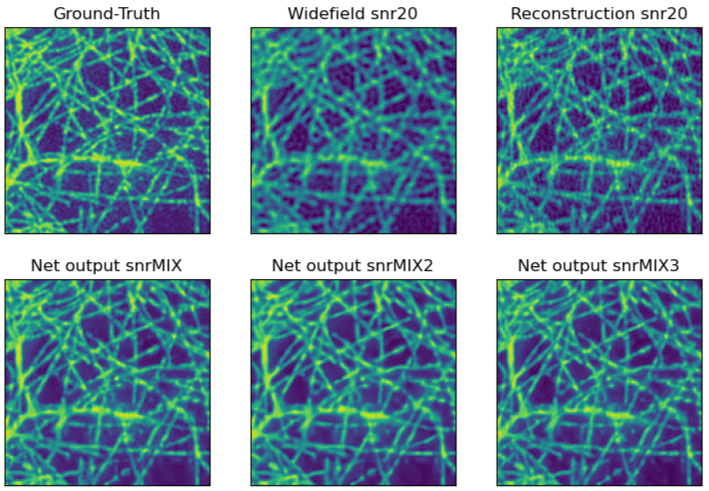
\includegraphics[width=0.48\textwidth]{images/test_img_2_model_comp_snr20.png}
    \caption{Visual comparison of widefield, reconstruction and the three DNN outputs in a zoomed region from test image 2 with SNR=20dB.}
    \label{fig:test_img_2_model_comp_snr20}
\end{figure}
\begin{figure}[h!]
    \centering
    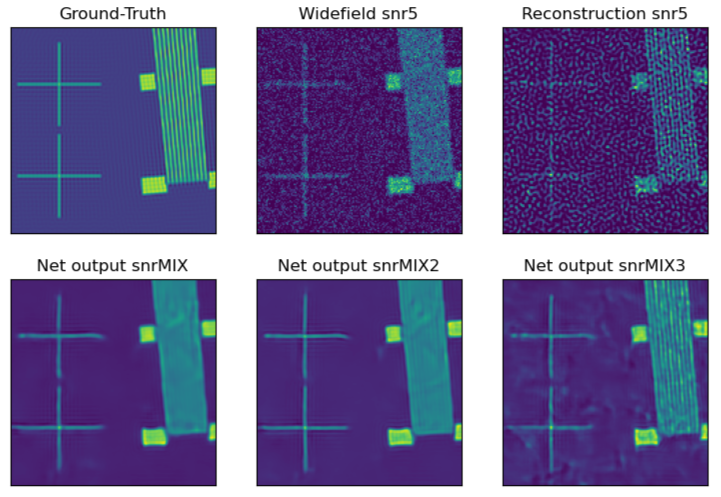
\includegraphics[width=0.48\textwidth]{images/test_img_3_model_comp_snr5_cross.png}
    \caption{Visual comparison of widefield, reconstruction and the three DNN outputs in a zoomed region (lines) from test image 3 with SNR=5dB.}
    \label{fig:test_img_3_model_comp_snr5_cross}
\end{figure}
\begin{figure}[h!]
    \centering
    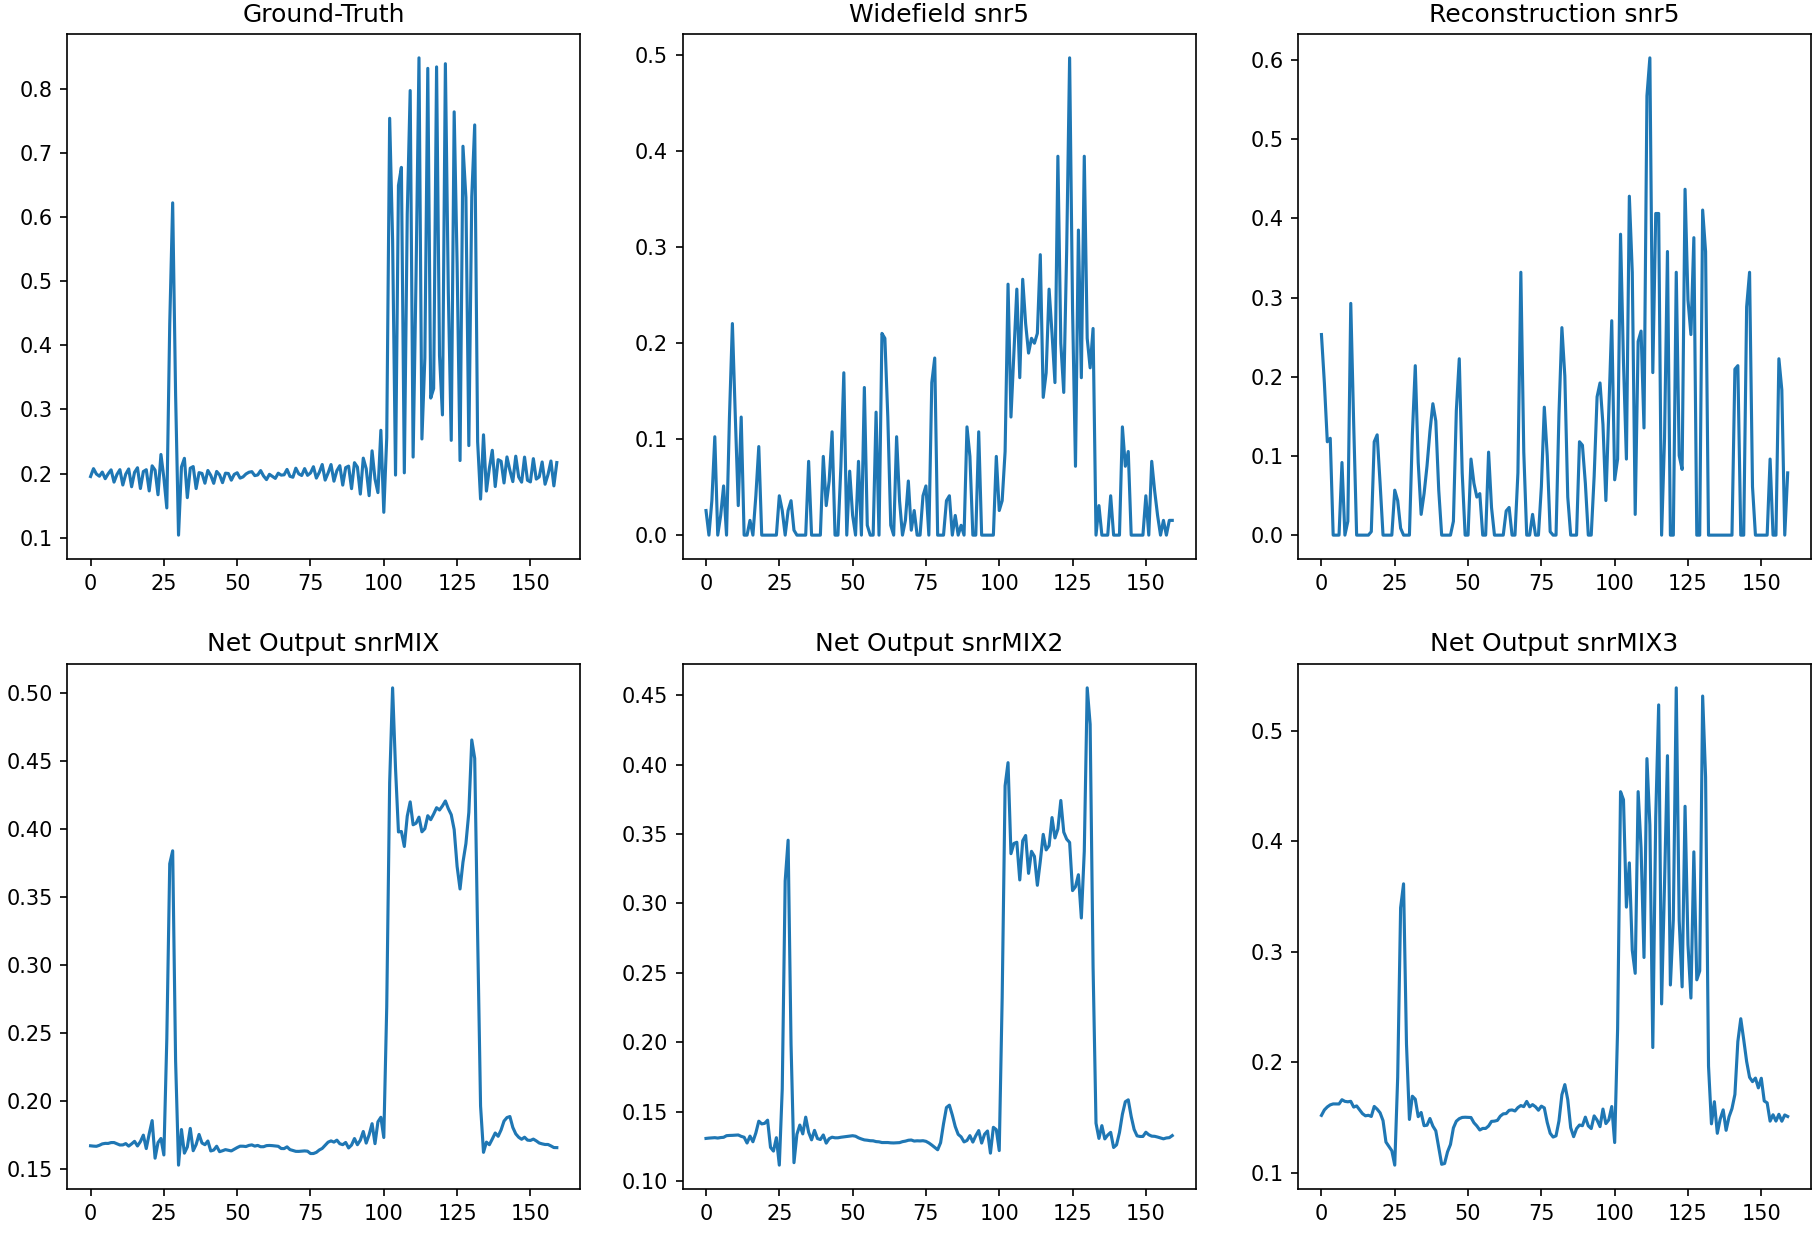
\includegraphics[width=0.48\textwidth]{images/test_img_3_model_comp_snr5_cross_cut.png}
    \caption{Intensity profile of a horizontal cut through the region visible in figure \ref{fig:test_img_3_model_comp_snr5_cross}.}
    \label{fig:test_img_3_model_comp_snr5_cross_cut}
\end{figure}
\begin{figure}[h!]
    \centering
    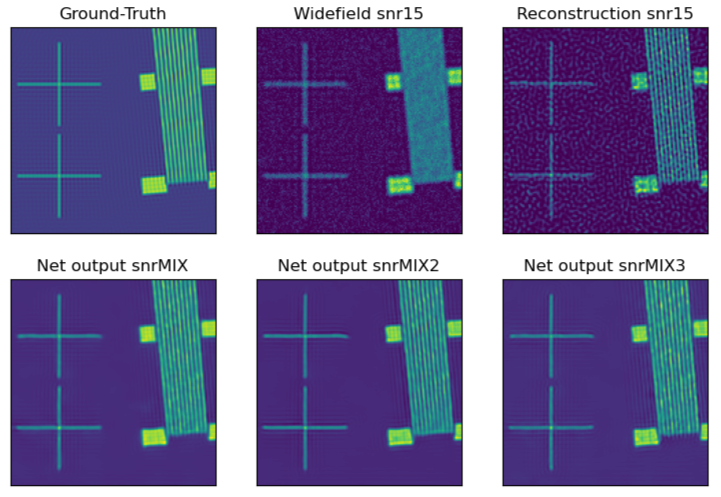
\includegraphics[width=0.48\textwidth]{images/test_img_3_model_comp_snr15_cross.png}
    \caption{Visual comparison of widefield, reconstruction and the three DNN outputs in a zoomed region (lines) from test image 3 with SNR=15dB.}
    \label{fig:test_img_3_model_comp_snr15_cross}
\end{figure}
\begin{figure}[h!]
    \centering
    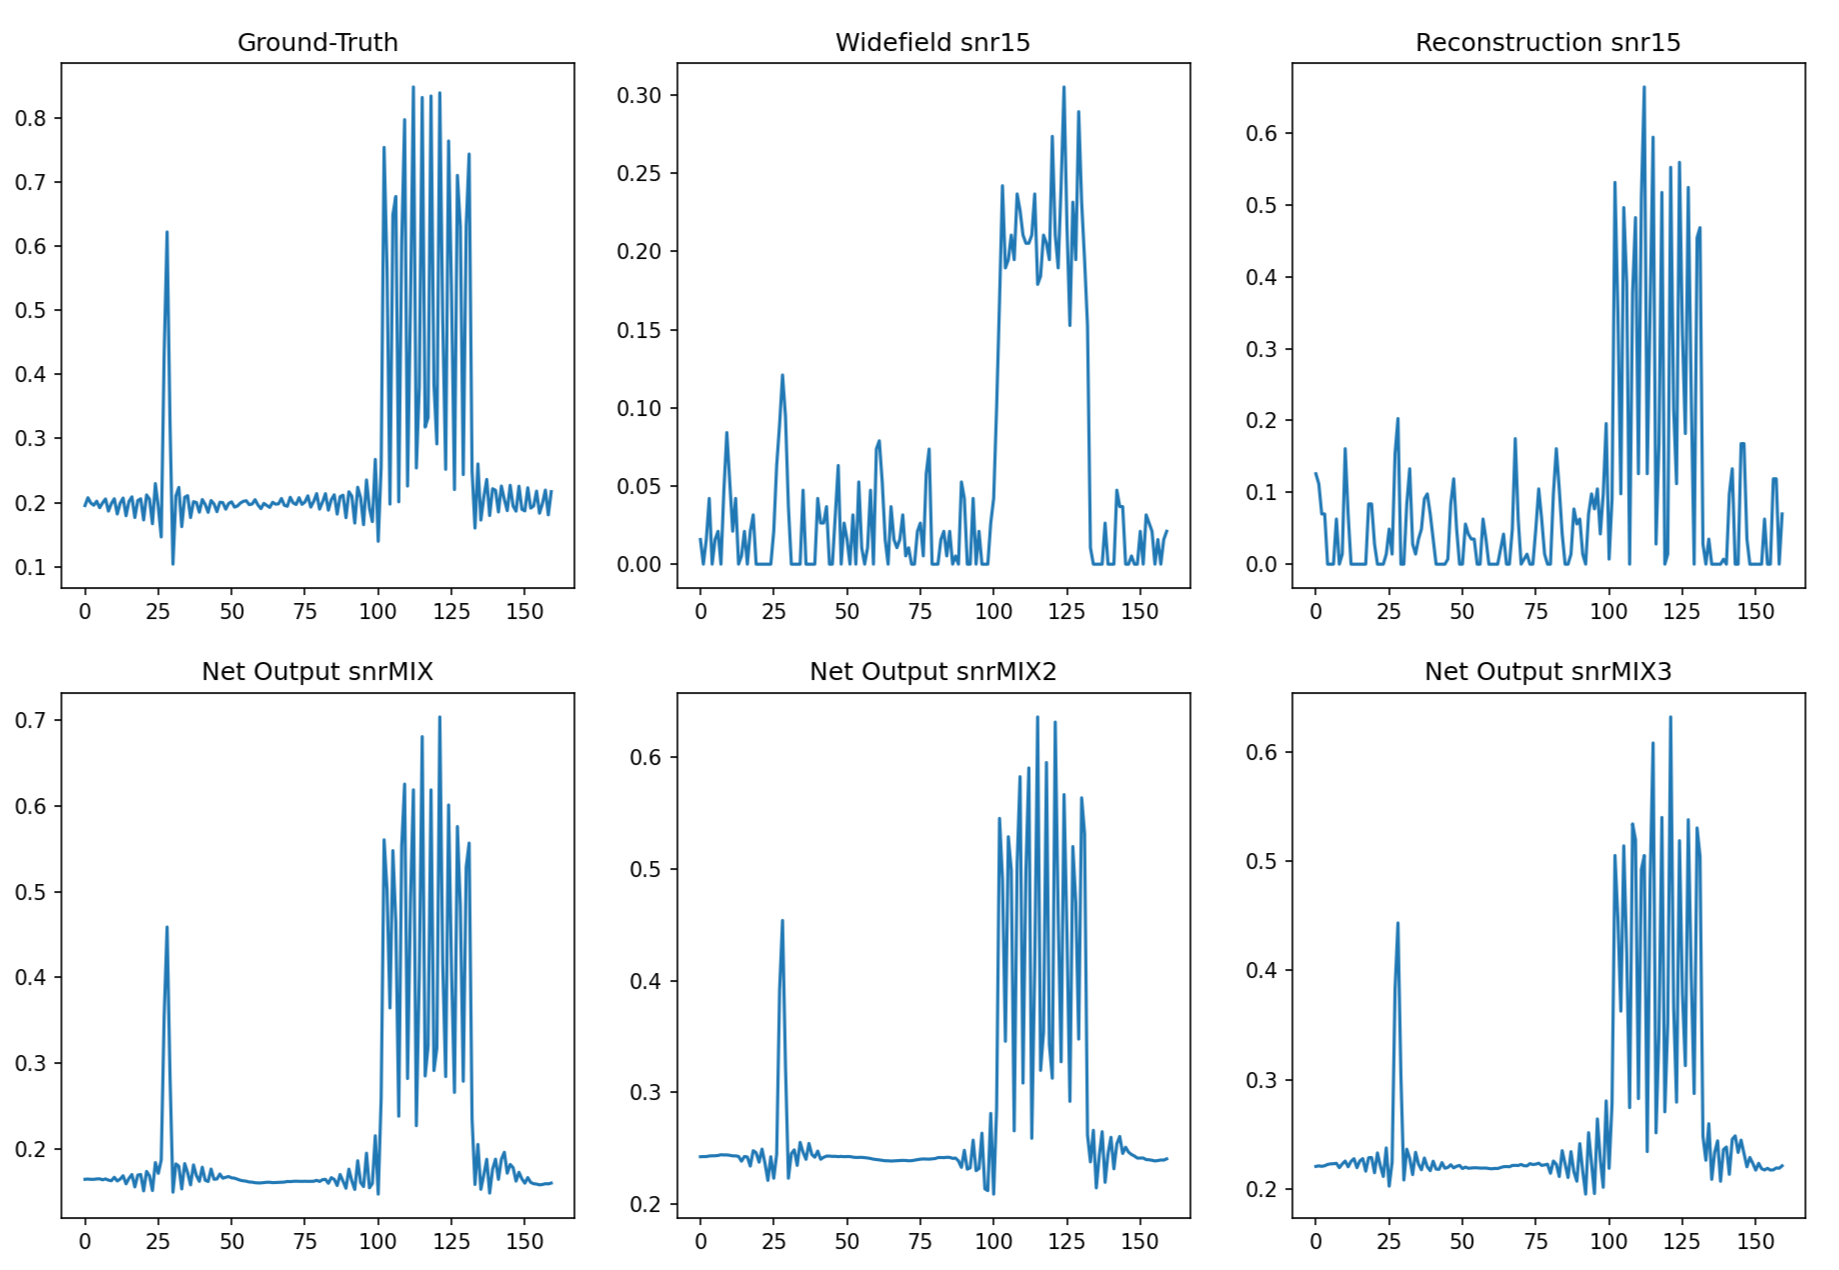
\includegraphics[width=0.48\textwidth]{images/test_img_3_model_comp_snr15_cross_cut.png}
    \caption{Intensity profile of a horizontal cut through the region visible in figure \ref{fig:test_img_3_model_comp_snr15_cross}.}
    \label{fig:test_img_3_model_comp_snr15_cross_cut}
\end{figure}
\begin{figure}[h!]
    \centering
    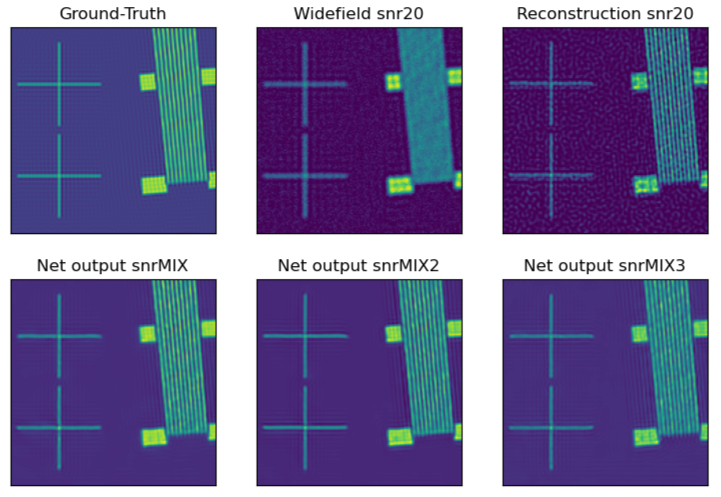
\includegraphics[width=0.48\textwidth]{images/test_img_3_model_comp_snr20_cross.png}
    \caption{Visual comparison of widefield, reconstruction and the three DNN outputs in a zoomed region (lines) from test image 3 with SNR=20dB.}
    \label{fig:test_img_3_model_comp_snr20_cross}
\end{figure}
\begin{figure}[h!]
    \centering
    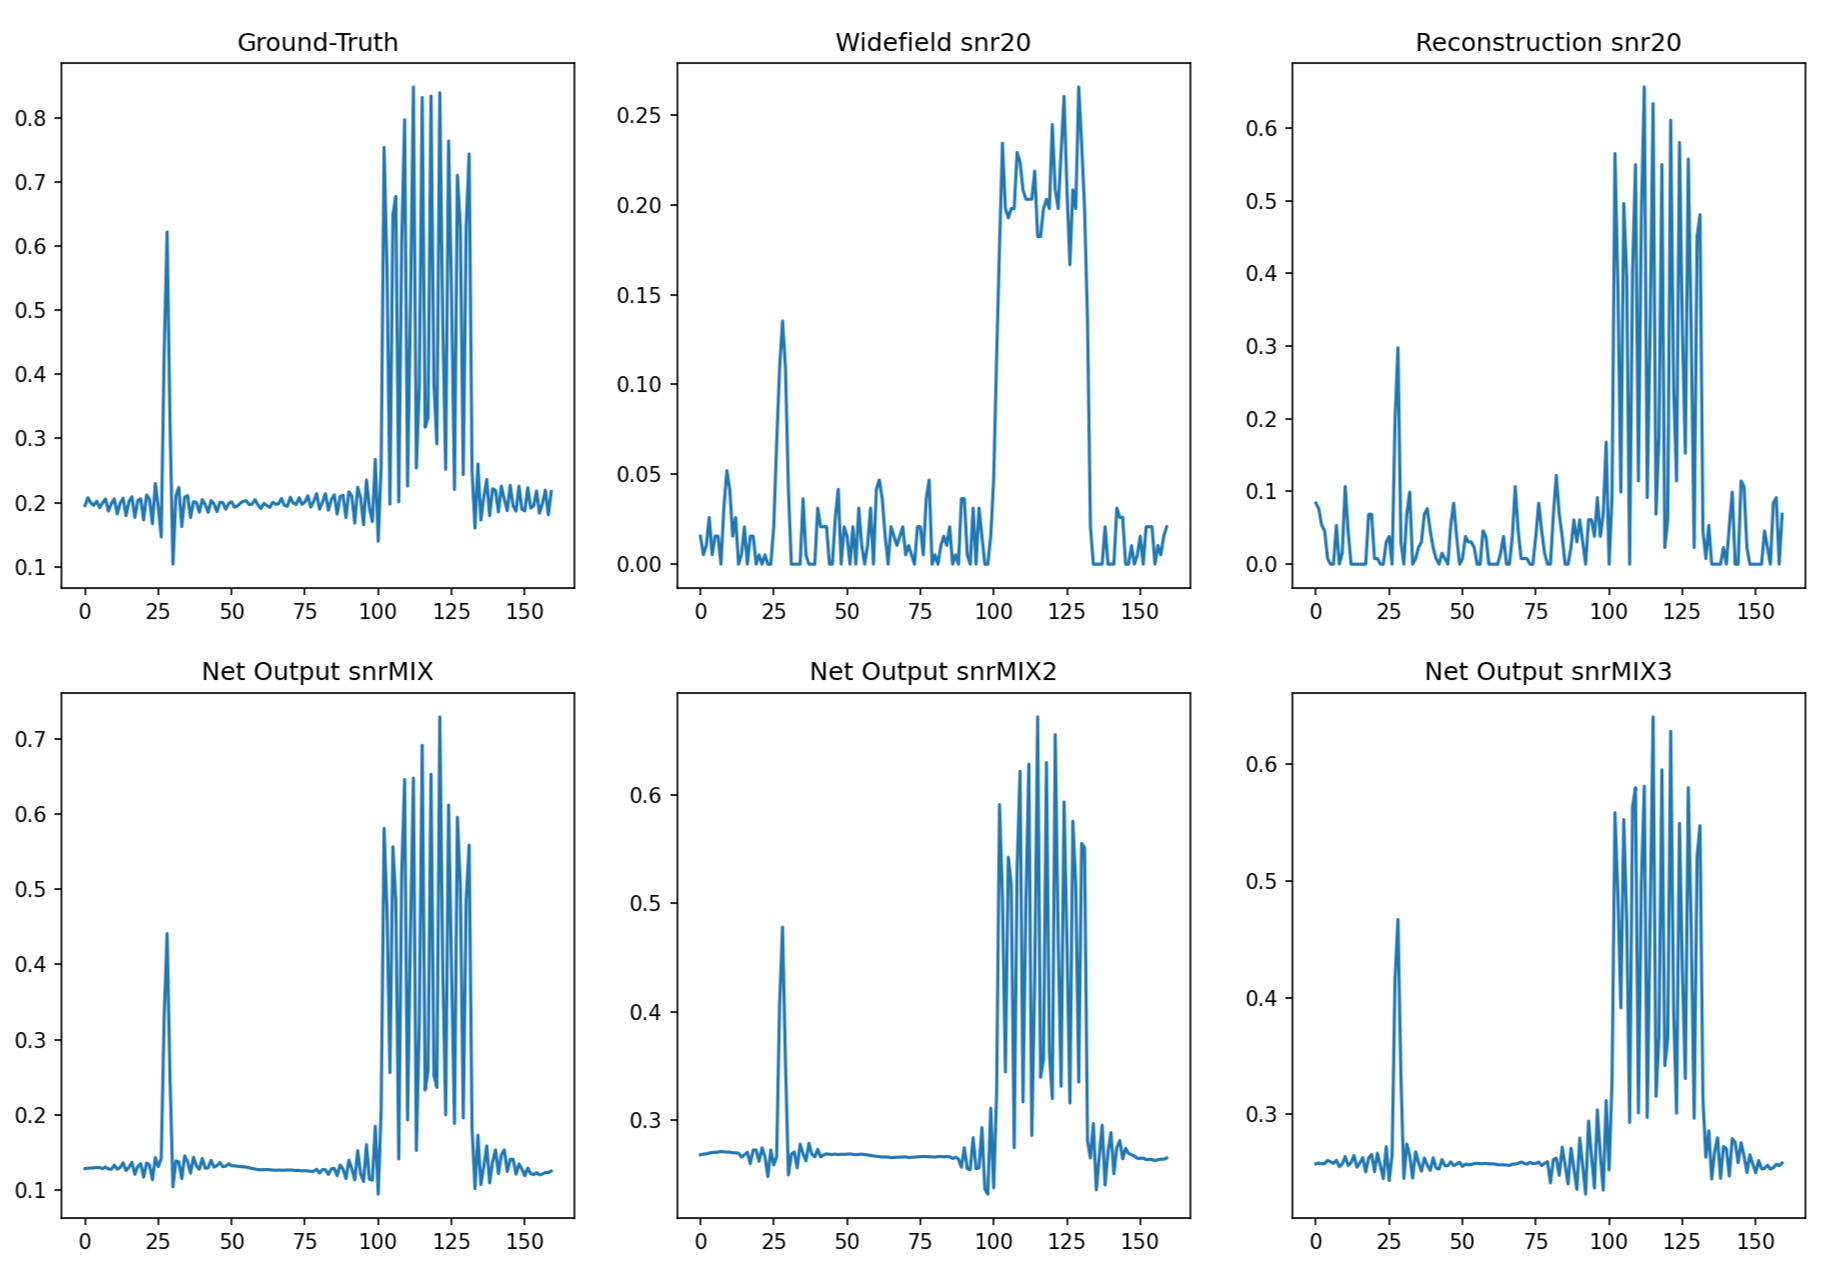
\includegraphics[width=0.48\textwidth]{images/test_img_3_model_comp_snr20_cross_cut.png}
    \caption{Intensity profile of a horizontal cut through the region visible in figure \ref{fig:test_img_3_model_comp_snr20_cross}.}
    \label{fig:test_img_3_model_comp_snr20_cross_cut}
\end{figure}
\begin{figure}[h!]
    \centering
    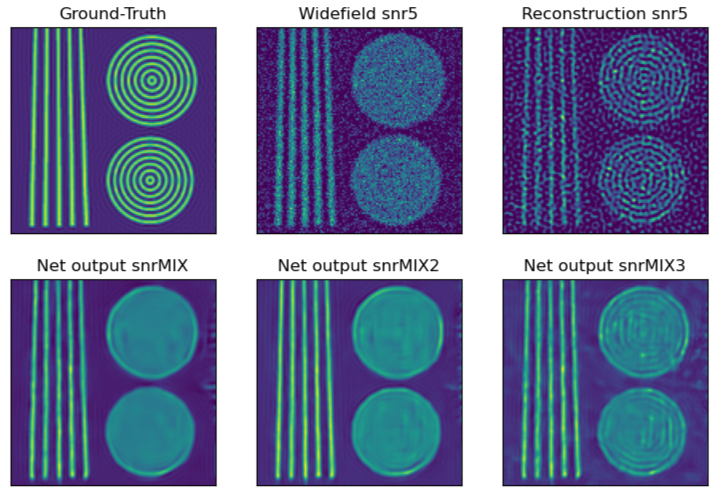
\includegraphics[width=0.48\textwidth]{images/test_img_3_model_comp_snr5_circle.png}
    \caption{Visual comparison of widefield, reconstruction and the three DNN outputs in a zoomed region (circles) from test image 3 with SNR=5dB.}
    \label{fig:test_img_3_model_comp_snr5_circle}
\end{figure}
\begin{figure}[h!]
    \centering
    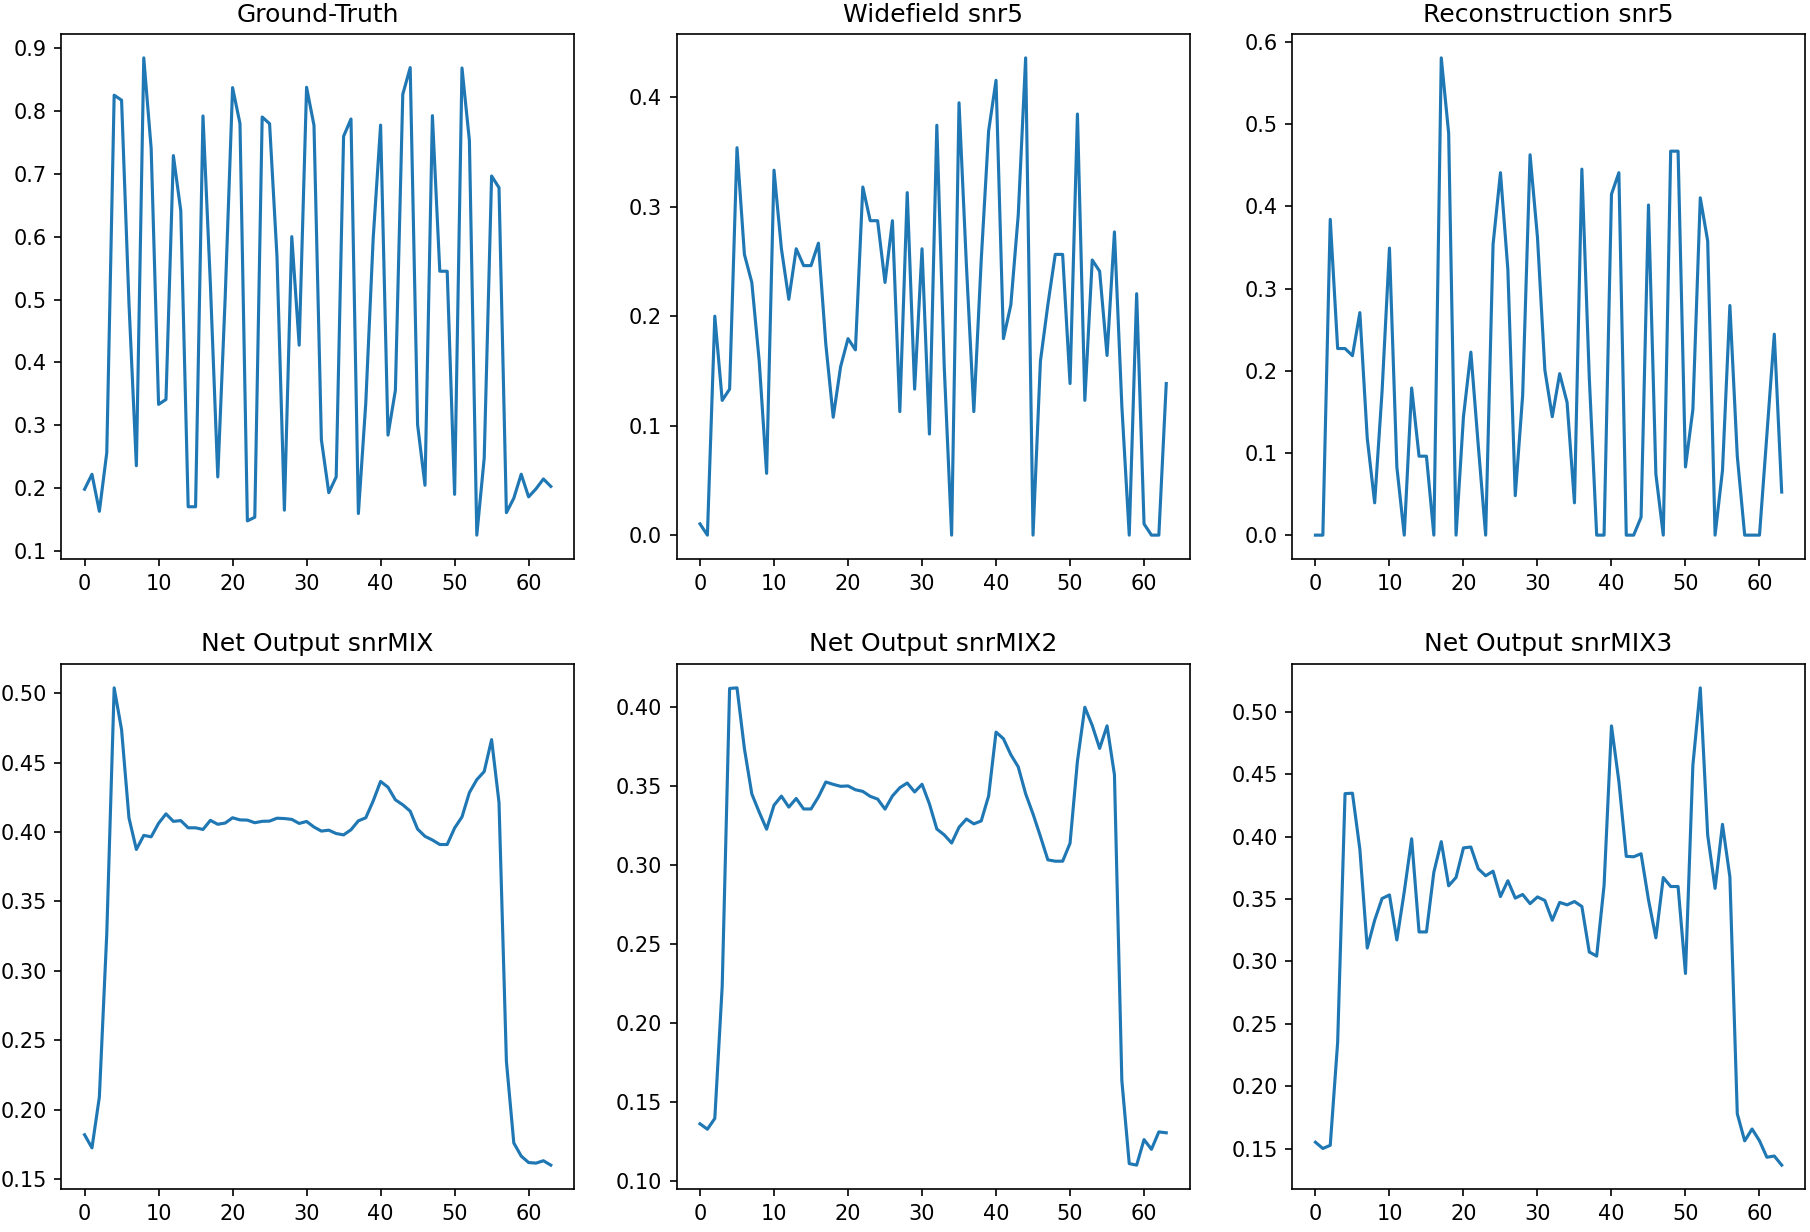
\includegraphics[width=0.48\textwidth]{images/test_img_3_model_comp_snr5_circle_cut.png}
    \caption{Intensity profile of a diagonal cut at 45$^\circ$ through the circles visible in figure \ref{fig:test_img_3_model_comp_snr5_circle}.}
    \label{fig:test_img_3_model_comp_snr5_circle_cut}
\end{figure}
\begin{figure}[h!]
    \centering
    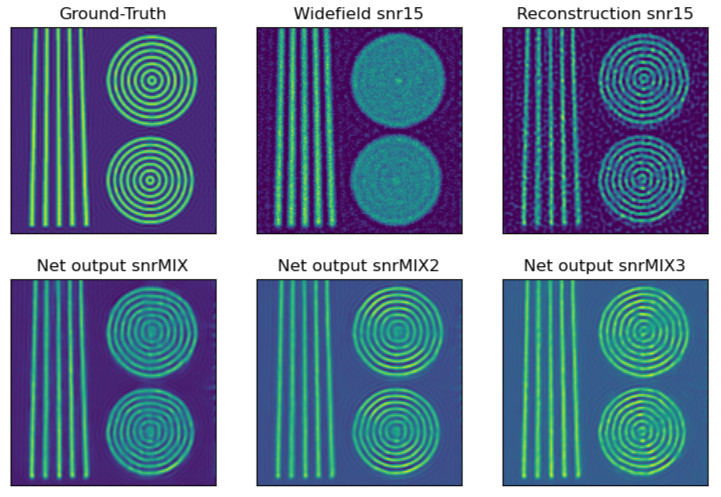
\includegraphics[width=0.48\textwidth]{images/test_img_3_model_comp_snr15_circle.png}
    \caption{Visual comparison of widefield, reconstruction and the three DNN outputs in a zoomed region (circles) from test image 3 with SNR=15dB.}
    \label{fig:test_img_3_model_comp_snr15_circle}
\end{figure}
\begin{figure}[h!]
    \centering
    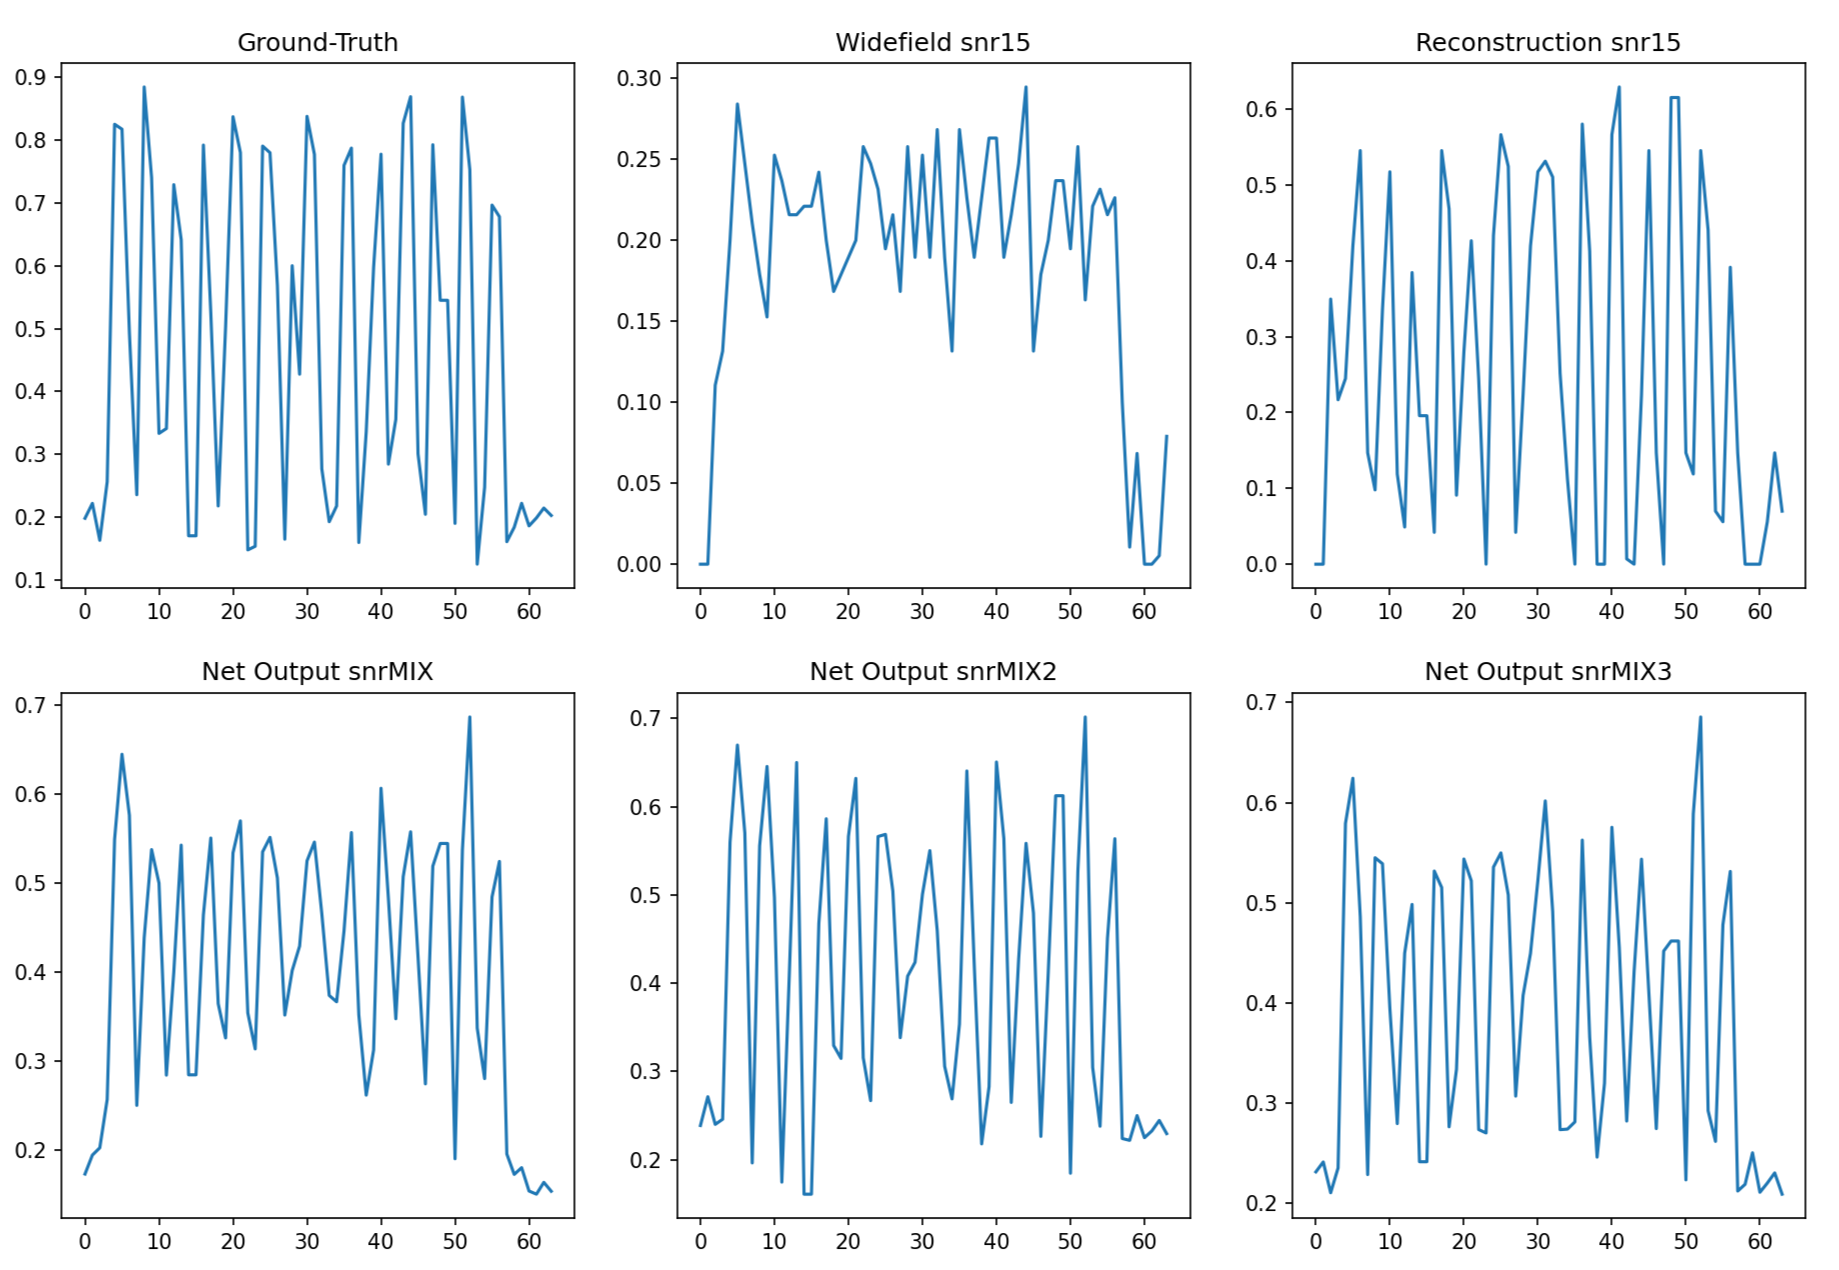
\includegraphics[width=0.48\textwidth]{images/test_img_3_model_comp_snr15_circle_cut.png}
    \caption{Intensity profile of a diagonal cut at 45$^\circ$ through the circles visible in figure \ref{fig:test_img_3_model_comp_snr15_circle}.}
    \label{fig:test_img_3_model_comp_snr15_circle_cut}
\end{figure}
\begin{figure}[h!]
    \centering
    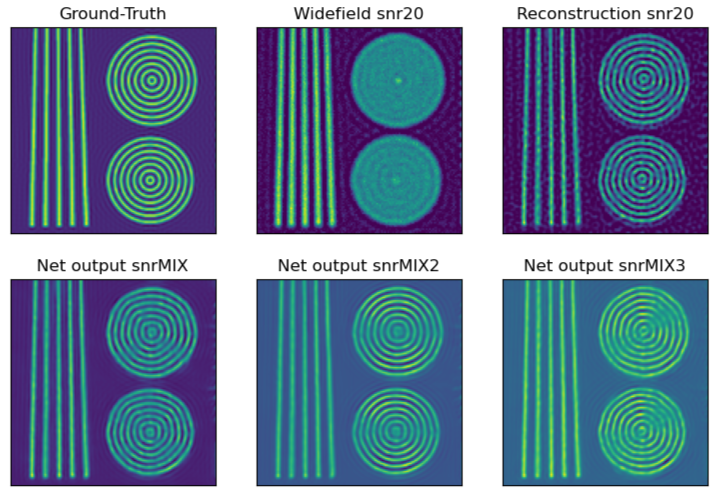
\includegraphics[width=0.48\textwidth]{images/test_img_3_model_comp_snr20_circle.png}
    \caption{Visual comparison of widefield, reconstruction and the three DNN outputs in a zoomed region (circles) from test image 3 with SNR=20dB.}
    \label{fig:test_img_3_model_comp_snr20_circle}
\end{figure}
\begin{figure}[h!]
    \centering
    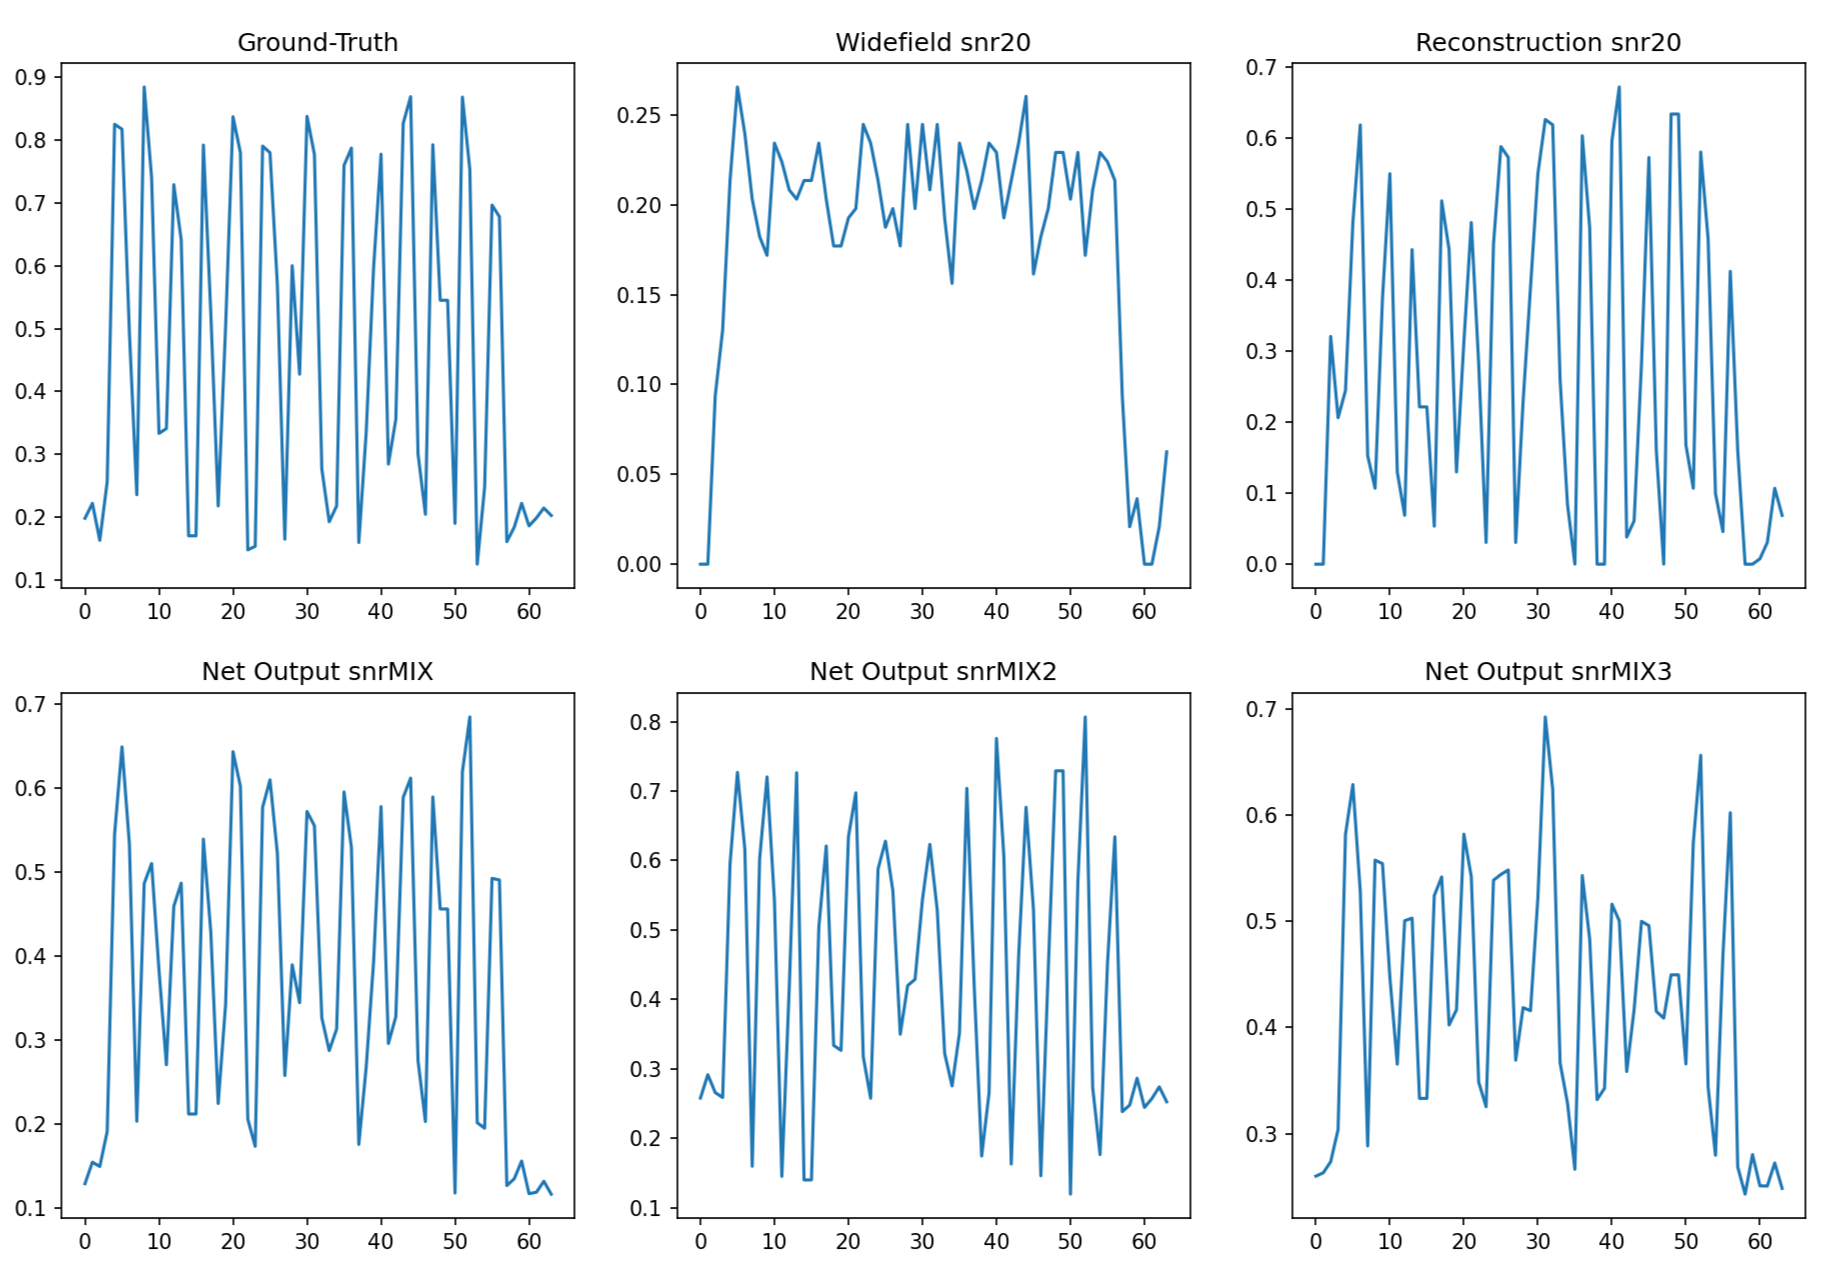
\includegraphics[width=0.48\textwidth]{images/test_img_3_model_comp_snr20_circle_cut.png}
    \caption{Intensity profile of a diagonal cut at 45$^\circ$ through the circles visible in figure \ref{fig:test_img_3_model_comp_snr20_circle}.}
    \label{fig:test_img_3_model_comp_snr20_circle_cut}
\end{figure}

\end{document}
